\documentclass[
  12pt, % Fontsize
  a4paper, % papersize
  oneside, % For twosided documents
  openany, 
  numbers=noenddot, % No final dots in Sectionnumbers, e.g 1.2 instead of 1.2.
  BCOR=5mm, % Correction length for lost space from binding
  parskip=half*, %No indent but spacing between paragraphs
  thesis, % type of document
]{bfhbook}


% Test Template for bfhbook.cls
\usepackage[T1]{fontenc}
% Coding 
\usepackage[utf8]{inputenc}
% Language setting
\usepackage[german]{babel}
\usepackage[export]{adjustbox}

% \usepackage{fonttable}
% Hyperref
\usepackage[                
  pdftex,                  % for PDF
  colorlinks=true,         % colored links
  linkcolor=black,         % color for links
  citecolor=black,         % color for references
  urlcolor=black,          % color for url 
  bookmarks=true
]{hyperref}              

\usepackage{booktabs} % For nicer tables
\usepackage{threeparttable} % Table-Captions having the same width than the table
\usepackage[singlelinecheck=off]{caption}
\usepackage{siunitx} % Scientific Units and number setting
\usepackage{listings} % For Program-Code
\usepackage{enumitem}

\usepackage{minted}
\setminted[arduino]{
    linenos=true,
    breaklines=true,
    encoding=utf8,
    fontsize=\footnotesize,
    xleftmargin=7mm
}
\setminted[shell]{
	frame=lines,
	framesep=5mm
}
\usemintedstyle{manni}

\usepackage{caption}
\captionsetup[figure]{font=footnotesize, labelfont=small}
\newcommand{\source}[1]{\caption*{Quelle: {#1}} }

\usepackage{xcolor}

\usepackage[export]{adjustbox}
\usepackage[document]{ragged2e} % left-alignment for text

\usepackage{glossaries}

% definition for directory tree with forest
\usepackage[edges]{forest}

\definecolor{foldercolor}{RGB}{124,166,198}

\tikzset{pics/folder/.style={code={%
    \node[inner sep=0pt, minimum size=#1](-foldericon){};
    \node[folder style, inner sep=0pt, minimum width=0.3*#1, minimum height=0.6*#1, above right, xshift=0.05*#1] at (-foldericon.west){};
    \node[folder style, inner sep=0pt, minimum size=#1] at (-foldericon.center){};}
    },
    pics/folder/.default={20pt},
    folder style/.style={draw=foldercolor!80!black,top color=foldercolor!40,bottom color=foldercolor}
}

\forestset{is file/.style={edge path'/.expanded={%
        ([xshift=\forestregister{folder indent}]!u.parent anchor) |- (.child anchor)},
        inner sep=1pt},
    this folder size/.style={edge path'/.expanded={%
        ([xshift=\forestregister{folder indent}]!u.parent anchor) |- (.child anchor) pic[solid]{folder=#1}}, inner xsep=0.6*#1},
    folder tree indent/.style={before computing xy={l=#1}},
    folder icons/.style={folder, this folder size=#1, folder tree indent=3*#1},
    folder icons/.default={12pt},
}

% end definition directory tree

%%%%%%%%%%%%%%%%%%%%%%%%%%%%%%%%%%%
% Settings 
%%%%%%%%%%%%%%%%%%%%%%%%%%%%%%%%
% Type?? (Lecture Notes, BSc Thesis, Master Thesis, . . .) 
% Use Variables \BSc, \Master, etc. for language support
\type{Semesterarbeit}
% Author(s)
\author{Marc Habegger}
% Title
\title{IoT Erfassung und Darstellung Sensordaten}
% Short Title, will be used in the footline
\shorttitle{CAS BGD Semesterarbeit}
% Subtitle
\subtitle{CAS Big Data}
% Titlepicture
\titlepicture{Bilder/Titel.png}
%%

% Topic of Study
\degreeprogramme{CAS Big Data}
% Expert
\expert{Max Kleiner}
% Version
\version{1.0}
% Date
\date{\today} % Or any other possible date

% Departement
% Use Variable for language support
%\TI

% Semester
% Use Variable for language support
%\semester

% Logo(s)

% Colors
% Secondary Color for Graphics, Tables etc.
% Naming: BFH*Color*light|middle|dark, e.g. BFHGreendark, BFHBluelight, etc.
% Possible Color Values: Green, Blue, Purple, Brown 
\newcommand{\seccolor}{BFHLightGreen} 

\setcounter{secnumdepth}{4}
\setcounter{tocdepth}{4}

% Variablen für diese Arbeit
\newcommand{\compImgSize}{4cm}

% Glossar Einträge
\makeindex
\makeglossaries

\newglossaryentry{IoT}
{
    name=Internet of Things,
    description={deutsch Internet der Dinge, Bezeichnet ein loses Netzwerk in welcher beliebige elektronische Geräte untereinander vernetzt werden. Wir häufig im Zusammenhang mit Sensornetzwerken verwendet.\break 
    \url{https://de.wikipedia.org/wiki/Internet_der_Dinge}}
}

\newacronym[see={[Glossary:]{IoT}}]{iot}{IoT}{Internet of Things}

\newglossaryentry{HMAC}
{
    name=Keyed-Hash Message Authentication Code,
    description={Verfahren zur Absicherung von gesendeten Nachrichten welches mit einer Hash-Funktion und einem geheimen Schlüssel arbeitet.\break
    \url{https://de.wikipedia.org/wiki/Keyed-Hash_Message_Authentication_Code}}
}

\newacronym[see={[Glossary:]{HMAC}}]{hmac}{HMAC}{Keyed-Hash Message Authentication Code}

\newglossaryentry{MQTT}
{
    name=Message Queuing Telemetry Transport,
    description={Offenes Nachrichtenprotokoll für Machine-to-Machine-Kommunikation (M2M), das die Übertragung von Telemetriedaten in Form von Nachrichten zwischen Geräten ermöglicht.\break
    \url{https://de.wikipedia.org/wiki/MQTT}}
}

\newacronym[see={[Glossary:]{MQTT}}]{mqtt}{MQTT}{Message Queuing Telemetry Transport}

\newglossaryentry{ARDUINO}
{
 	name=Arduino,
    description={Arduino ist eine aus Soft- und Hardware bestehende Physical-Computing-Plattform. Beide Komponenten sind im Sinne von Open Source quelloffen.\break
    \url{https://de.wikipedia.org/wiki/Arduino_(Plattform)}}
}

\newglossaryentry{ZIGBEE}
{
	name=ZigBee,
    description={ZigBee ist eine Spezifikation für drahtlose Netzwerke mit geringem Datenaufkommen.\break
    \url{https://de.wikipedia.org/wiki/ZigBee}}
}

\begin{document}

\maketitle
%**************************************************************************
%\frontmatter % preliminary parts

\tableofcontents
\sloppy
%%%%%%%%%%%%%%%%%%%%%%%%
% Introduction
%**************************************************************************
\mainmatter % The main part
%**************************************************************************
%\part{Part One}
\chapter*{Management Summary}
Das Internet der Dinge (\Gls{iot}) zeichnet sich, neben einer allgegenwärtigen Verfügbarkeit von Daten, auch durch eine grosse Anzahl der Datenquellen aus. Mit dieser Arbeit soll das Zusammenspiel der verschiedenen Komponenten eines Sensornetzwerkes mit einem Speichersystem und einer grafischen Analyse aufgezeigt werden.

  \begin{center}\label{overview}
    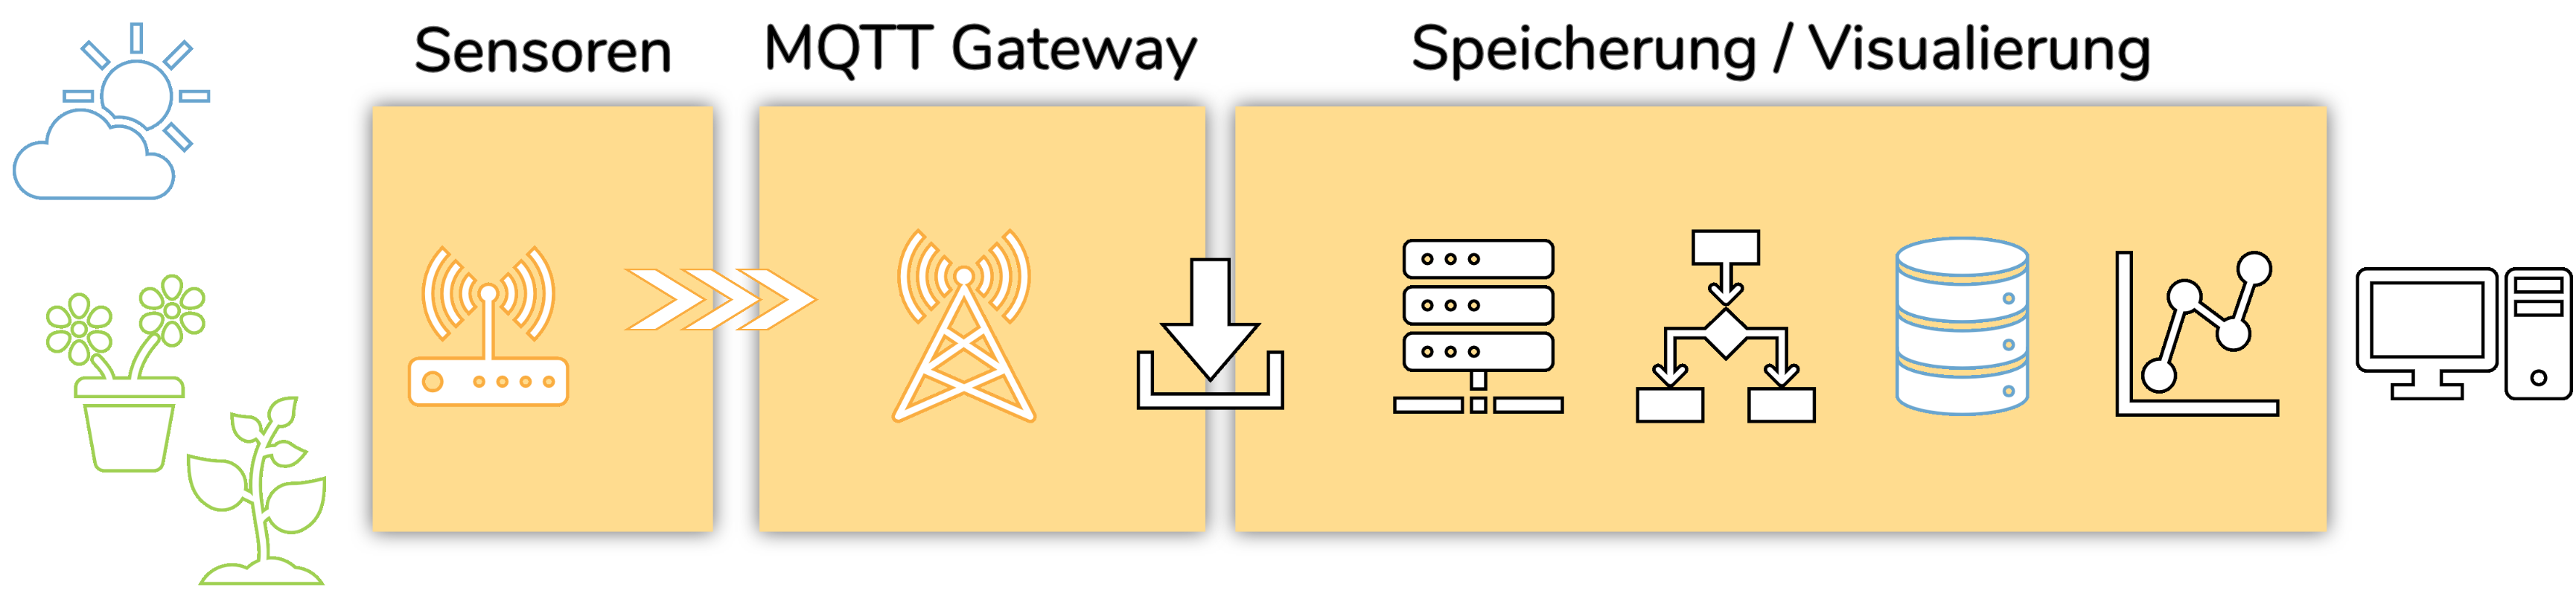
\includegraphics[width=18cm, left]{Bilder/Overview.png}
     \captionsetup{justification=centering}
      \captionof{figure}{Systemaufbau Funknetzwerk}
  \end{center}
   
Das realisierte Netzwerk besteht aus mehreren Sensoren, die Messdaten über Funk an ein MQTT-Gateway senden, welches über ein Netzwerk mit einer Datenbank verbunden ist. Für die Speicherung der Daten wird eine Zeitreihendatenbank verwendet, die speziell für die Behandlung von Messwerten optimiert ist.

  \begin{center}
    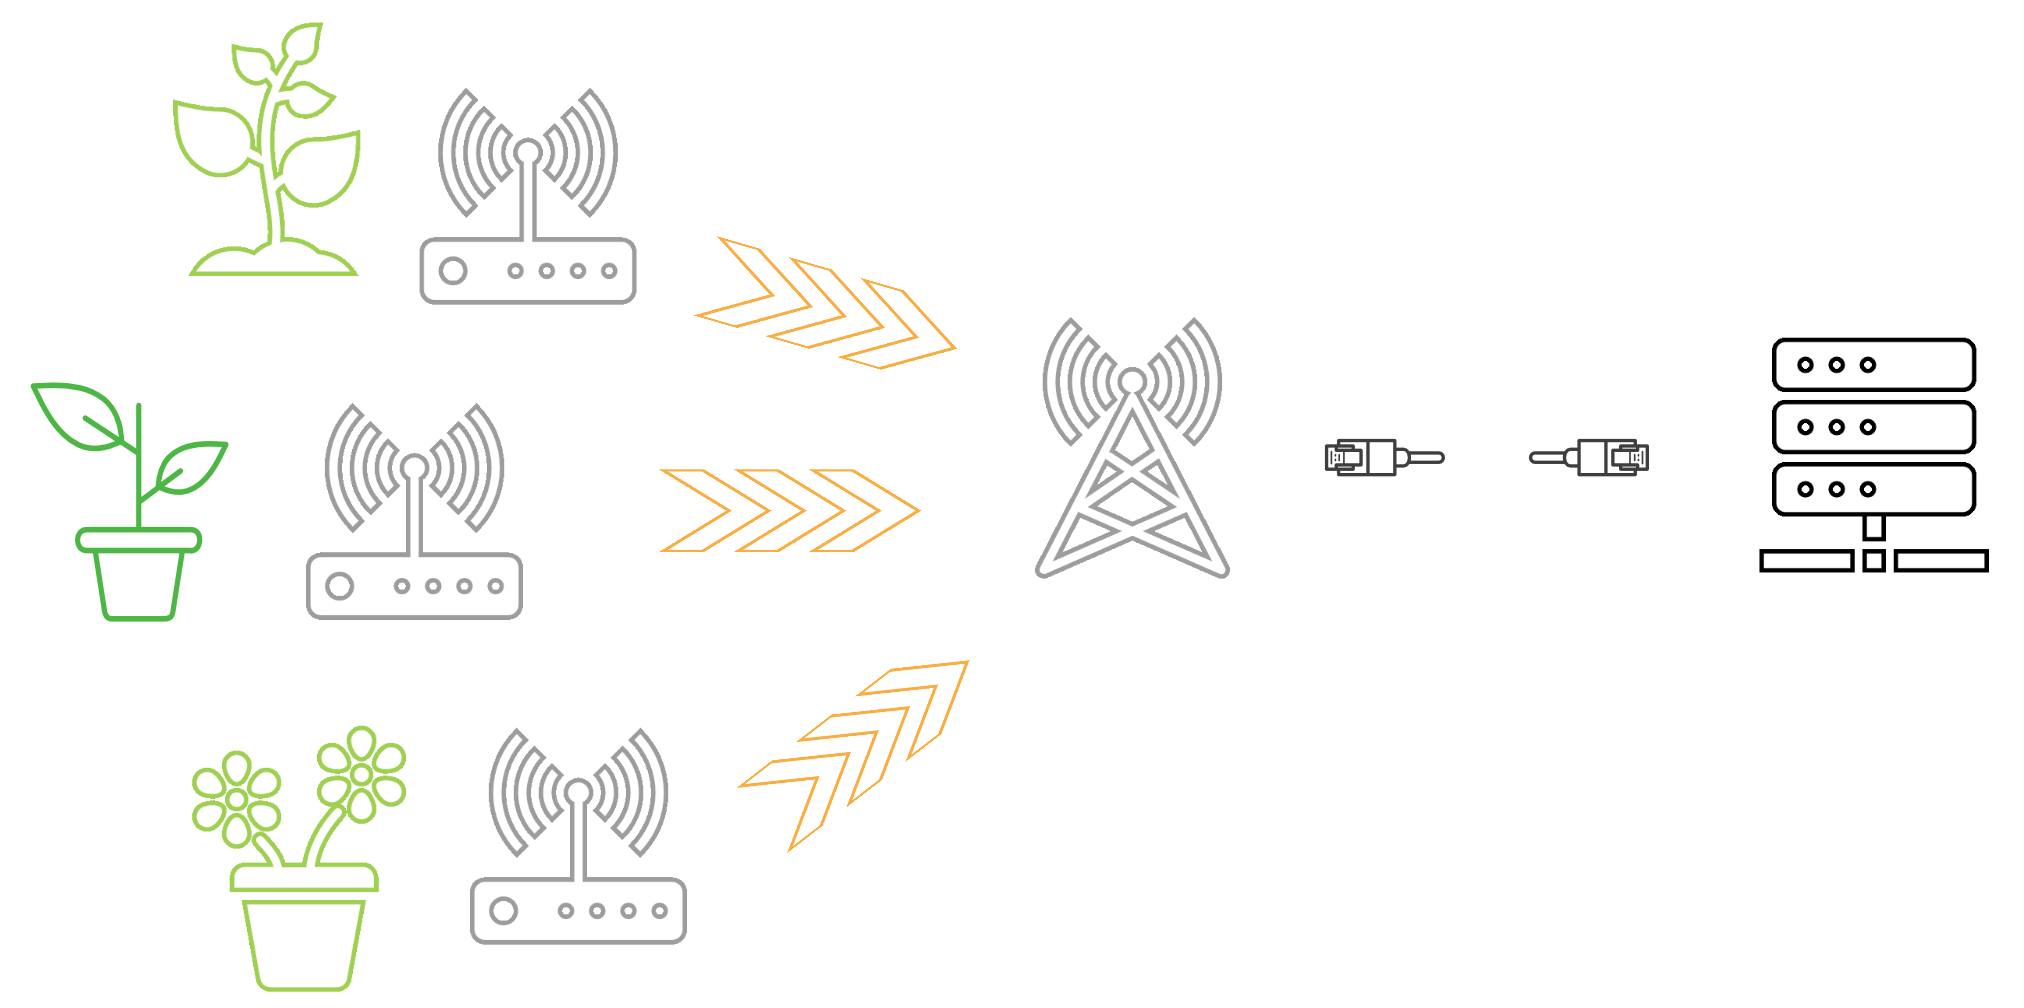
\includegraphics[width=14cm, left]{Bilder/Overview-2.png}
     \captionsetup{justification=centering}
      \captionof{figure}{Systemaufbau}
  \end{center}
  Schlussendlich werden die Daten visualisiert und können über einen Browser betrachtet werden. Beim erreichen oder unterschreiten selbst definierter Schwellwerte kann ein Alarm ausgelöst werden.
\chapter{Einleitung}
Der gesamte Code und die Dokumentation dieser Arbeit ist auf Github unter folgendem Link zu finden:

 \url{https://github.com/habis-git/CAS-BGD-SemesterArbeit} 
 
 und wird auch nach Abschluss dieser Arbeit weiterentwickelt. Die Komponenten wurden durch das Vorhandensein von Bibliotheken und Treibern, sowie die leichte Beschaffung auch innerhalb der Schweiz, ausgewählt. Der Arduino Mega als MQTT Gateway und der Raspberry Pi 2 für die Linux Plattform waren bereits von früheren Projekten vorhanden und wurden deshalb in diesem Projekt eingesetzt.

Der Aufbau dieses Dokumentes folgt der Übersichtsgrafik  \ref{overview} mit den Sensoren auf der linken Seite und der Visualisierung auf der Rechten Seite und dementsprechend werden die Sensoren zuerst beschrieben und die Visualisierung findet sich gegen Ende des Dokumentes.

Diese Dokumentation hat nicht den Anspruch den Aufbau des Projektes in jedem Punkt zu erläutern, gewisse Arbeiten wie z. Bsp. Lötarbeiten oder auch Konfigurationen auf Betriebssystem Ebene fehlen. Die Übersicht der Webseiten [\ref{links}] welche die nötigen Informationen für dieses Projektes lieferten, kann bei solchen Fragen weiterhelfen.

Das ursprüngliche LaTeX Template für dieses Dokument stammt aus diesem Projekt:

\url{https://gitlab.ti.bfh.ch/bfh-latex/bfh-latex}

\chapter{Sensor Plattform}
\section{Mikrokontroller}
Ein sehr beliebter Mikrokontroller ist der ESP32 von Espressif \cite{espressif}, welcher durch grossen Funktionsumfang und geringem Preis überzeugen kann. Ein Vorteil ist ebenfalls die Möglichkeit der Programmierung durch die Arduino\cite{arduino} IDE, welche frei verfügbar ist und die Entwicklung stark vereinfacht. Es existieren viele verschiedene Mikrocontroller, welche den ESP32 Baustein verwenden. Für dieses Projekt kam der Firebeetle \cite{firebeetle} von DF Robot zum Einsatz.
\begin{center}
\begin{minipage}[t]{0.5\linewidth}
	\centering
	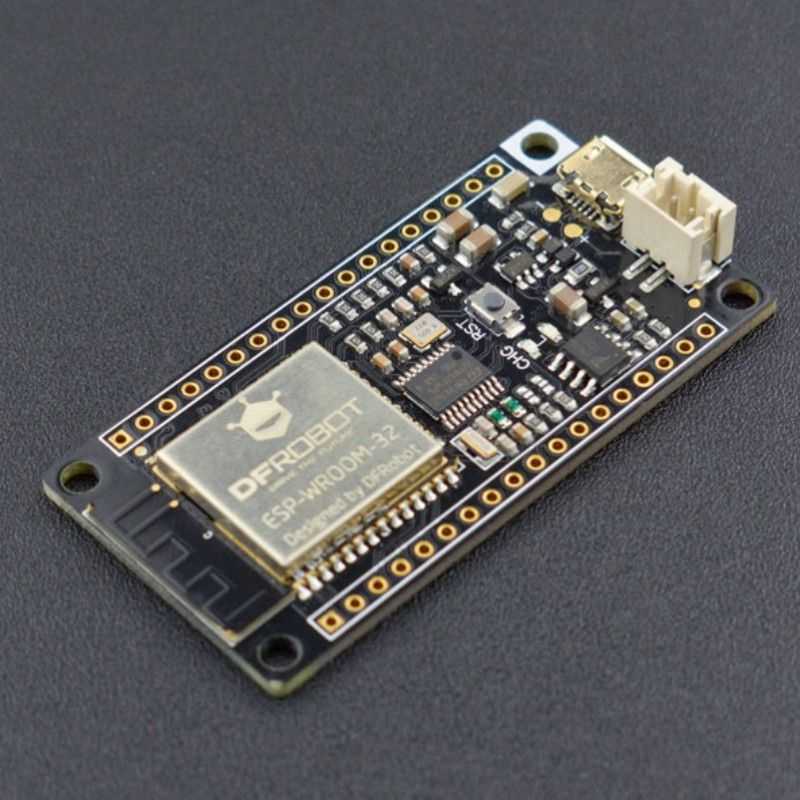
\includegraphics[ width=0.75\linewidth, valign=t]{Bilder/Firebeetle.jpg} 
	 \captionof{figure}{Firebeetle mit dem ESP32 Mikrokontroller}
\end{minipage}%
\begin{minipage}[t]{0.5\linewidth}
Der ESP32 besitzt sowohl WLAN als auch Bluetooth LE Schnittstellen. Diese wurden jedoch aus Gründen des Stromverbrauchs (WLAN) oder der Reichweite (Bluetooth LE) in diesem Projekt nicht verwendet.\break \break
 Der Firebeetle\cite{firebeetle} Baustein hat sowohl die Möglichkeit einer Stromversorgung mit 5 Volt, als auch mit 3.7 Volt, womit er direkt durch Lithium-Ionen Akkus betrieben werden kann.
\end{minipage}
\end{center}
\section{Funkverbindung}
Die Wahl der Funktechnologie wurde nach folgenden Punkten getroffen:
\begin{itemize}
	\item Stromverbrauch (je kleiner desto besser)
	\item Reichweite (20-30 m für die Anwendung im Garten)
	\item Preis
	\item Verfügbarkeit von Bibliotheken für die Programmierung
\end{itemize}

\begin{table}[t]
\renewcommand{\arraystretch}{2} % In order to set the correct linespacing.
% Must be set here, since this also changes the linespacing for the array
% environment
\arrayrulecolor{white}
	\begin{center}
		\rowcolors{1}{\seccolor!10}{\seccolor!10} % Rows with 10% of secondary color
% See page 33 of the "BFH Markenmanual"
	\begin{threeparttable}
	\begin{tabular}{lllll}
	%	\toprule
		\rowcolor{\seccolor!50}
		& NRF24 & ZigBee & Bluetooth LE & WLAN\\\bfhmidline
		Frequenz &  2.4 GHz & 868/915 MHz \& 2.4 GHz & 2.4 GHz & 2.4–5 GHz   \\\bfhmidline
		Stromverbrauch & 18 mA & 30–40 mA & 30-15 mA & 116-22 mA \\\bfhmidline  
		Benötigte Leistung & 60 mW & 36.9 mW & 215 mW-10 mW & 835 mW-200 mW \\\bfhmidline
		Reichweite  & 10–50 m & 10–300 m & 10–30 m & 100–500 m
		%\bottomrule
	\end{tabular}
	\caption{Leistung der verschiedenen Funktechniken im Vergleich}\label{tab:radioTable}
	 \source{Design of Wireless Sensors for IoT with Energy Storage and Communication Channel Heterogeneity \cite{radioPower}}
	\end{threeparttable}
	\end{center}
\end{table}
Aus der Tabelle \ref{tab:radioTable} geht hervor, dass die ZigBee Technologie ein attraktives Paket aus geringem Stromverbrauch und guter Reichweite bietet. Allerdings sind die Module für ZigBee relativ kostspielig (20-30 Fr.), womit sich jeder einzelne Sensor stark verteuert. Bluetooth LE ist zwar ebenfalls sehr stromsparend, dies allerdings nur in der kürzesten Reichweite (>10m), welche für dieses Projekt unzureichend ist.

Schussendlich war es die Kombination aus guter Reichweite, sehr geringem Stromverbrauch und extrem günstigem Preis (< 2 Fr.) bei den NRF24 Modulen, die überzeugte.

\section{Sensoren}
 Es existiert eine grosse Anzahl an verschiedenen Sensoren, welche auch für Privatanwender nutzbar sind. In diesem Projekt wurden Sensoren gewählt für welche frei verfügbare Bibliotheken in einer Version für den ESP32 vorhanden sind. Grundsätzlich wird bei den Sensoren unterschieden zwischen solchen die 
 \begin{itemize}
	 \item Digitale Werte liefern, die direkt einer Einheit (Grad Celsius) oder Prozentangabe (Luftfeuchtigkeit) entsprechen
	  \item Analoge Messwerte, welche auf eine Einheit umgerechnet werden müssen
\end{itemize}
Für dieses Projekt wurden mehrere Sensoren ausgewählt und kombiniert:
\begin{itemize}
	\item Lufttemperatur- und Luftfeuchtigkeitssensoren DHT11 [\ref{DHT11}] und DHT22 [\ref{DHT22}]
	\item Bodenfeuchtesensor V1.2 [\ref{moistV1.2}]
\end{itemize}
\section{Aufbau}
Die Komponenten werden alle mit den 3.7 Volt und Masse Anschlüssen verbunden. Das Funkmodul benötigt die SPI Kontakte SCK, MOSI und MISO und zusätzlich zwei digitale Pins für CE und CSN, die frei gewählt werden können. In meinem Code habe ich CE auf den Pin 25 gesetzt und CSN auf Pin 26. Wenn man andere Pins verwenden möchte, dann kann dies bei der Initialisierung des Funkmoduls angegeben werden: \mint{arduino}|radio = new RF24(25, 26); //CE, CSN|

Der Daten-Input des Temperatur Sensors benötigt einen digitalen Eingang, welchen ich auf den Pin 27 gesetzt habe. Der Bodenfeuchtigkeitssensor hat einen analogen Ausgang, welchen ich mit Pin 4 verbunden habe. Für andere Pins können die folgenden Variablen angepasst werden:
\begin{minted}{arduino}
// DHT Sensor
uint8_t DHTPin = 27;
// Moisture Sensor
uint8_t MOISTSENSOR_PIN = 4;
\end{minted}
Die Schaltung kann über den Mikro-USB Anschluss oder einen Lithium-Ionen-Akku mit Strom versorgt werden. Wenn ein Akku direkt angeschlossen werden soll, hat es auf der Rückseite  unterhalb des USB Anschlusses zwei Lötaugen. Ein so angeschlossener Akku kann danach über die USB Buchse geladen werden, der ESP32 enthält zu diesem Zweck eine Lade-Elektronik.

  \begin{center}
    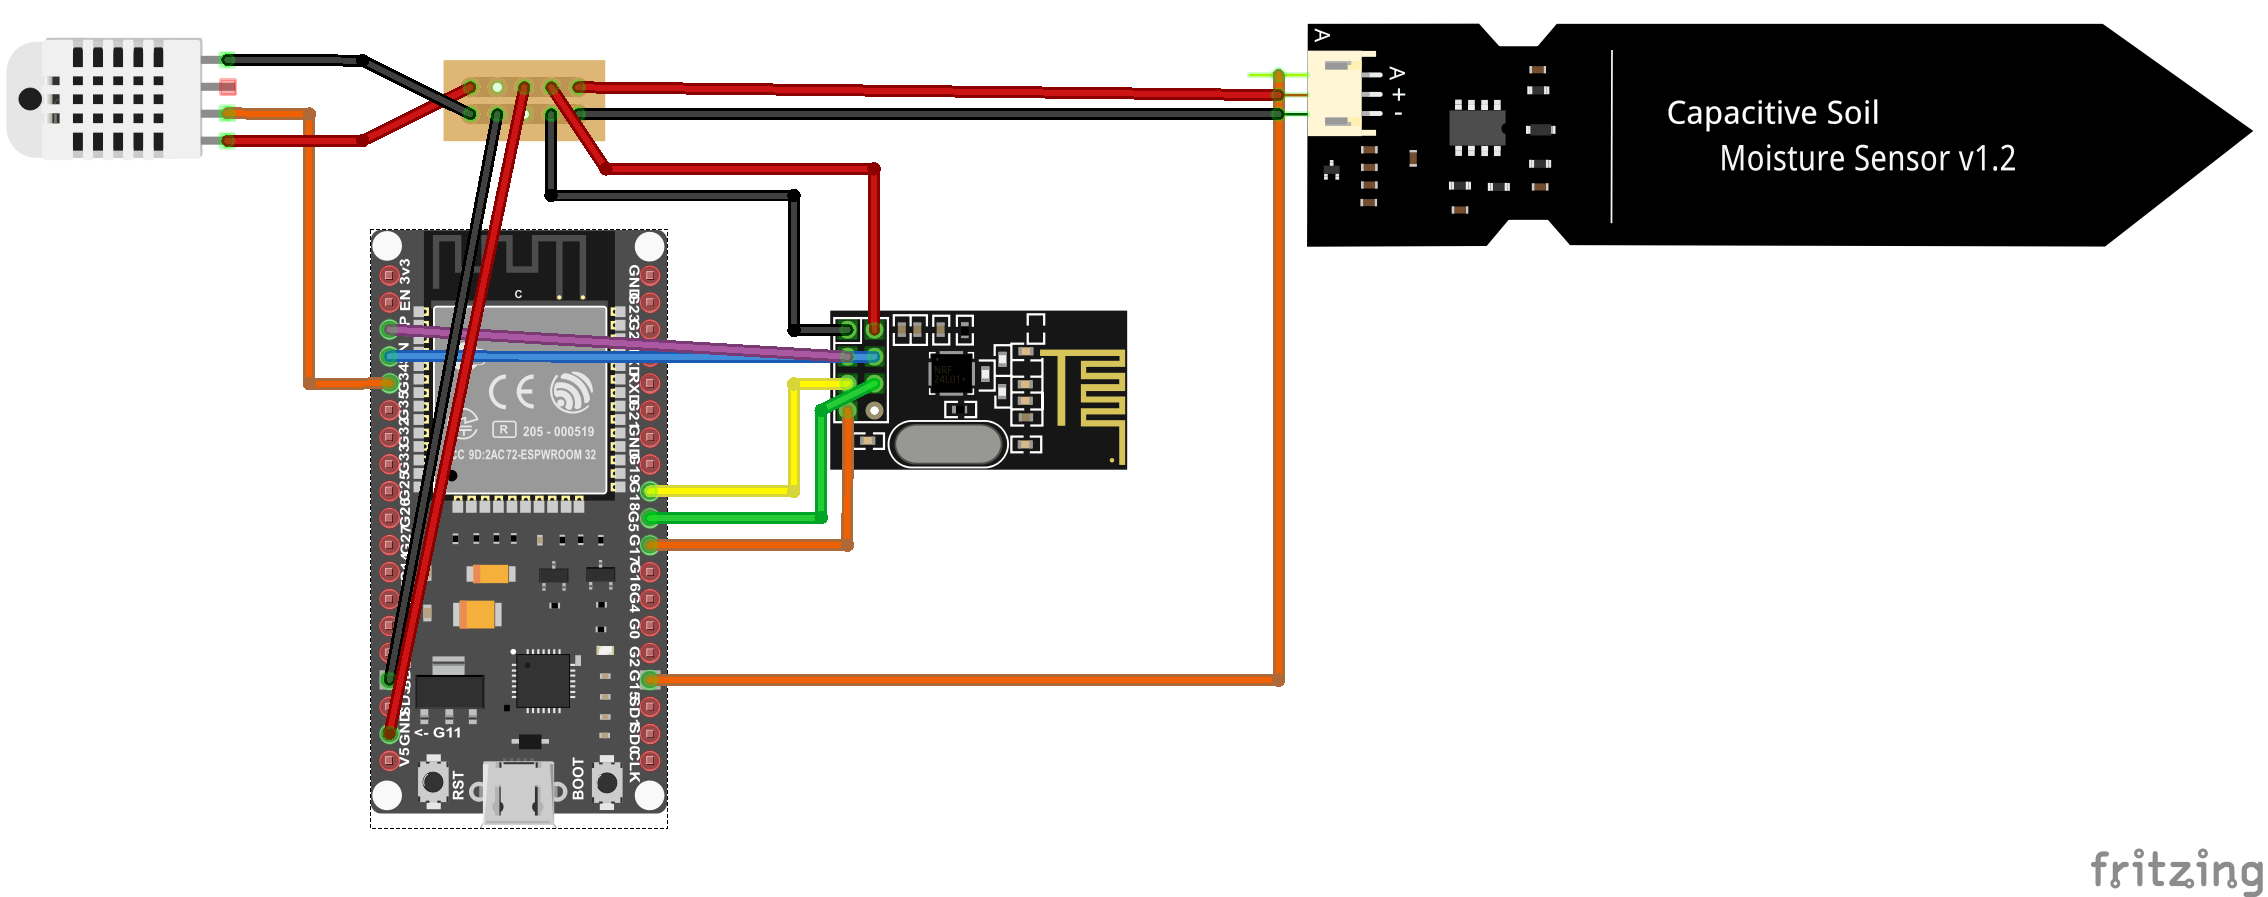
\includegraphics[width=17cm, left]{Bilder/Sensor-Design_Steckplatine.png}
    \captionsetup{justification=centering}
    \captionof{figure}{Verdrahtung der Komponenten}
   \end{center}


 \section{Funkverbindung mit dem MQTT Gateway}
 Da die Sensoren nicht WLAN als Funktechnik verwenden, können sie nicht direkt auf den MQTT Server verbinden und diesem Nachrichten senden. Diese Aufgabe übernimmt das MQTT-Gateway, welches auf der einen Seite ebenfalls mit einem NRF24 [\ref{nrf24}] Funkmodul ausgerüstet ist und andererseits eine Ethernet Netzwerkanbindung hat.
 
 Jedes Funkmodul kann mit 5 anderen Modulen kommunizieren, dabei muss jedes Modul eine eigene Adresse verwenden unter der es senden und empfangen kann.
\begin{center}
    \begin{minipage}[b]{0.45\textwidth}
        \centering
        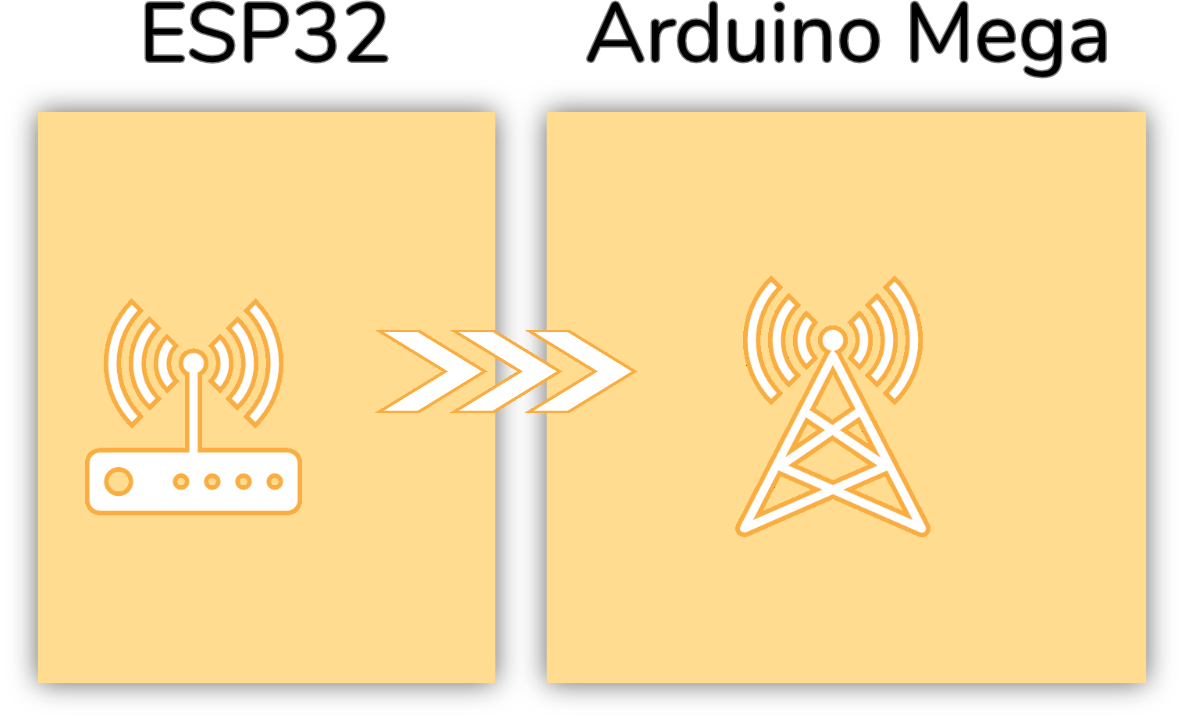
\includegraphics[width=7cm]{Bilder/ESP32-Arduino.png} % first figure itself
        \captionsetup{justification=centering}
        \captionof{figure}{Funkverbindung}
    \end{minipage}\hfill
    \begin{minipage}[b]{0.45\textwidth}\label{nrf24}
        \centering
        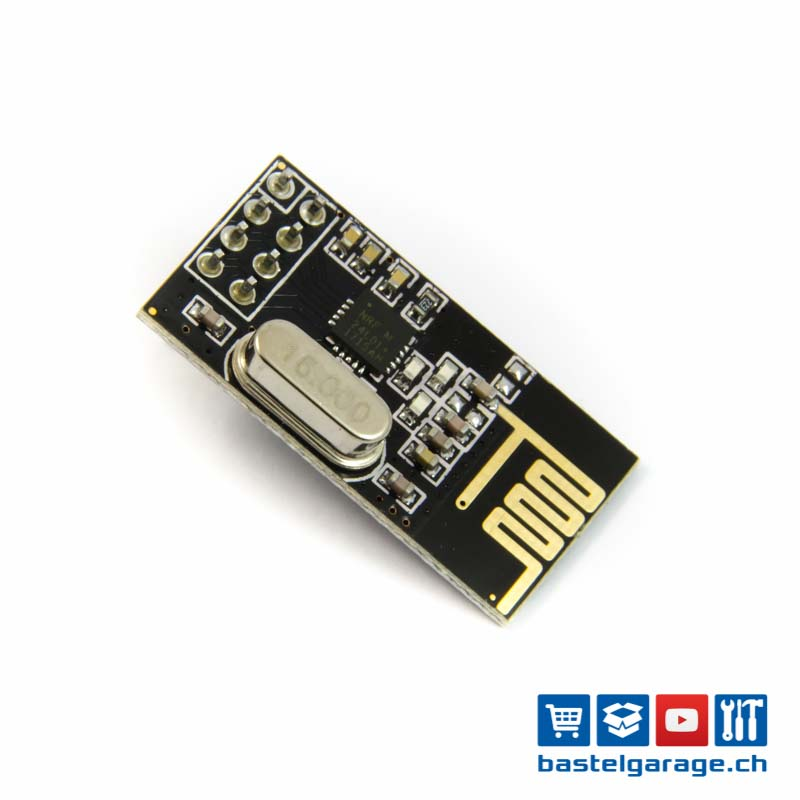
\includegraphics[width=\compImgSize]{Bilder/NRF24.jpg} % second figure itself
        \captionsetup{justification=centering}
        \captionof{figure}{NRF24L01+ Funkmodul}
    \end{minipage}
\end{center}
Bei der Programmierung der Sensoren wurde darauf geachtet, dass die Identifikation der Sensoren über eine einzigartige Id unabhängig vom Programmcode vorgenommen werden kann [\ref{config}].
\begin{center}
    \begin{minipage}[b]{0.45\textwidth}
        \centering
        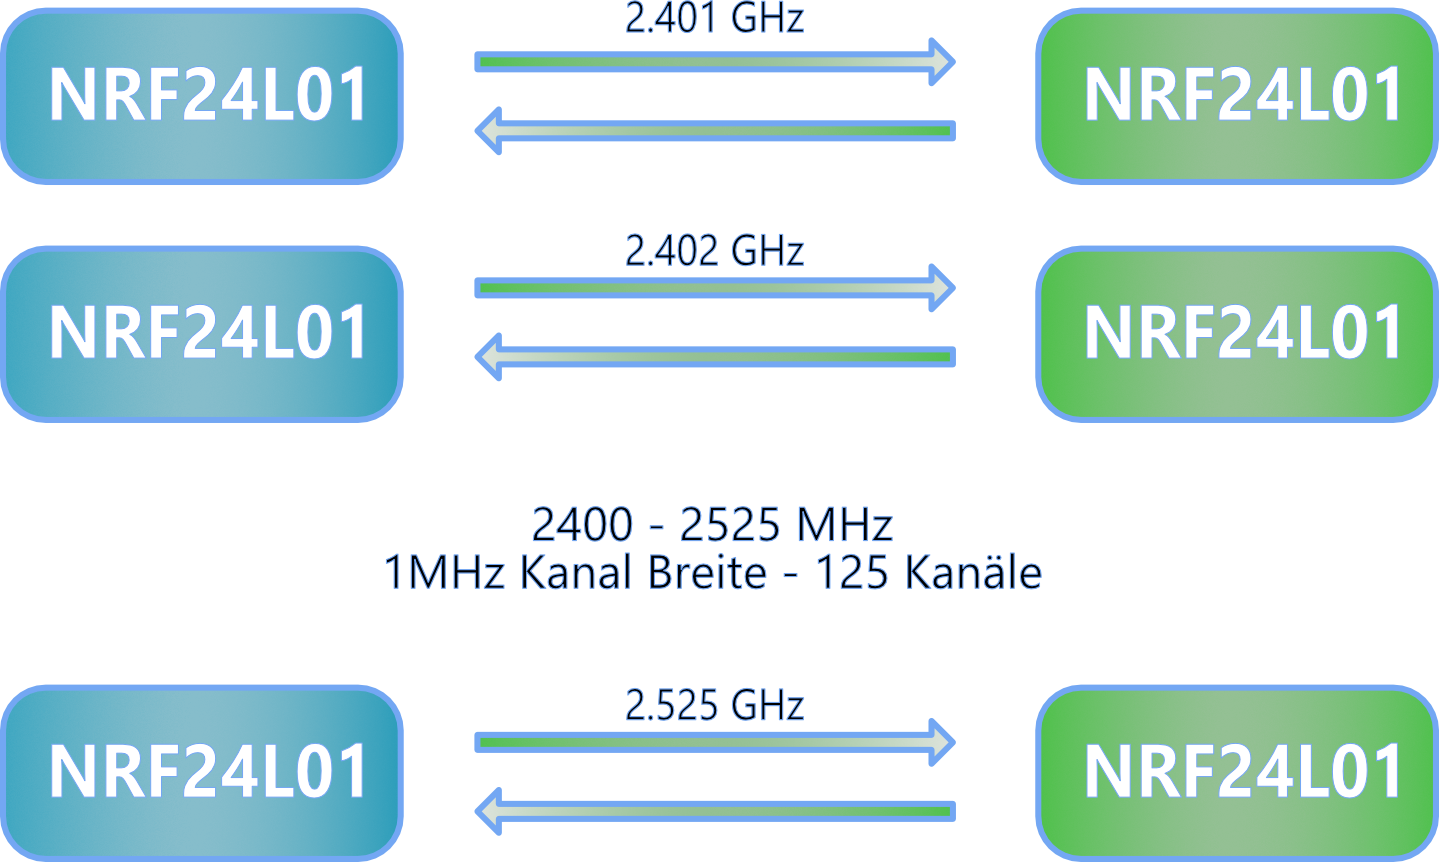
\includegraphics[width=9cm]{Bilder/NRF24Kommunikation.png}
        \captionsetup{justification=centering}
        \captionof{figure}{Funkkanäle des NRF24L01}
    \end{minipage}\hfill
    \begin{minipage}[b]{0.45\textwidth}
        \centering
        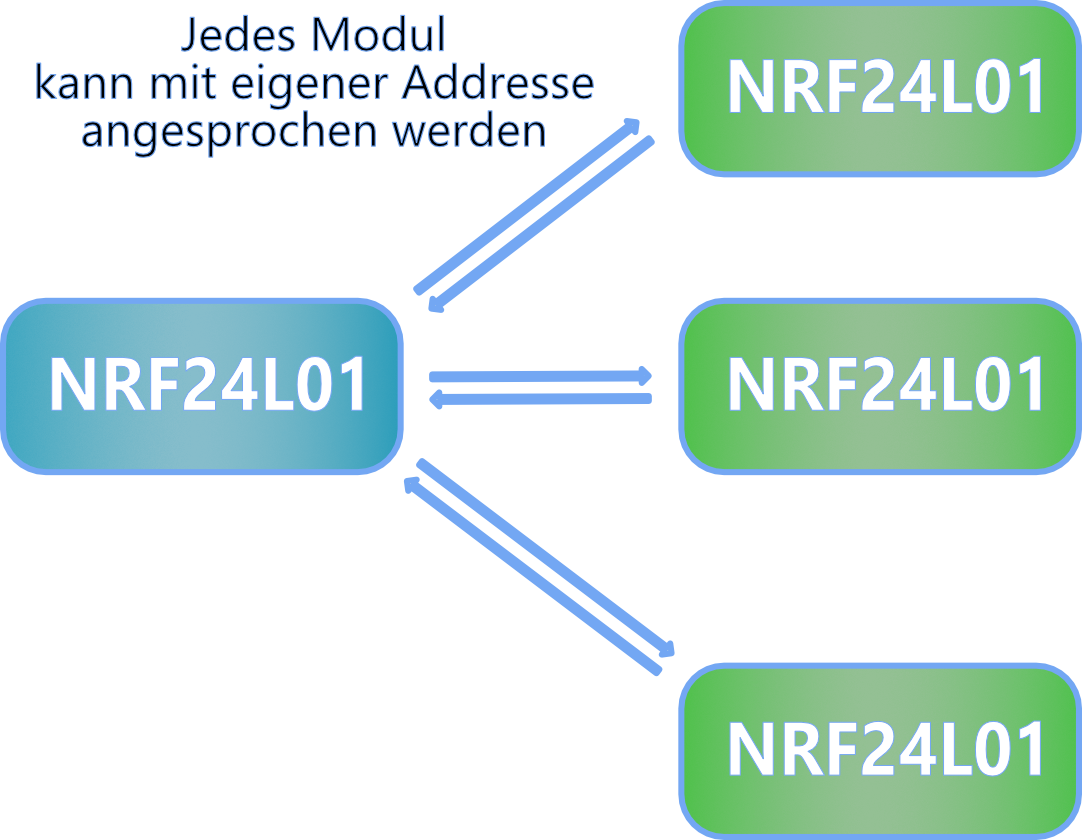
\includegraphics[width=7cm]{Bilder/NRF24Kommunikation-2.png} % second figure itself
        \captionsetup{justification=centering}
        \captionof{figure}{Addressierung Funkmodule}
    \end{minipage}
\end{center}
\subsection{Absicherung der Funkverbindung}\label{funkAbsicherung}
Die Identifikation eines Sensors ist aber nicht zu Verwechseln mit einer Prüfung ob der Sender überhaupt berechtigt ist Daten zu senden. Da das Funkprotokoll unverschlüsselt ist, können andere Sender ebenfalls Nachrichten absenden und so Daten verfälschen oder die Verarbeitung stören. Um dies zu verhindern, wird eine Technik Namens \Gls{hmac} eingesetzt.
Die eigentliche Nachricht \mint{html}| 4;25.1;71.1;10.2| wird dabei um einen Hash-Wert erweitert
\mint{html}|3A51266ABD432C1FB797DEDEE215FD16E42BAB627F104BCB6F4169EDE4544582:4;25.1;71.1;10.2| und die Nachricht mit \Gls{hmac} und den Messwerten wird an das \Gls{mqtt} Gateway geschickt.
 \section{Software}
 \subsection{Verwendete Bibliotheken}

  \begin{description}
\item[SPI library] Ansteuerung der Sensoren \cite{spi}
\item[mbed TLS] Berechnung des \Gls{hmac} \cite{mbedTLS}
\item[RF24] Funkmodul \cite{nrf24}
\item[DHT-sensor-library] Luft- und Feuchtigkeitssensor \cite{dht}
 \end{description}
Einige der aufgeführten Bibliotheken können direkt über die Bibliotheksverwaltung der Arduino IDE installiert werden. Ansonsten können die Bibliotheken über den Link (führt meistens auf github.com) heruntergeladen und von Hand installiert werden. 
{\color{red}Achtung: Es gibt viele Bibliotheken mit ähnlichem Namen und Beschreibung. Falls das kompilieren fehlschlägt bitte prüfen, ob die richtige Bibliothek eingebunden wurde.}

 \subsection{Konfiguration eines Sensors}\label{config}
\begin{center}
    \begin{minipage}[b]{0.45\textwidth}
       Der Flash-Speicher des ESP32 kann in mehrere Bereiche unterteilt werden. So können Dateien unabhängig von dem kompilierten Programm auf den Mikrocontroller geladen werden. Während der Programm-Code während der Entwicklung ständig ändert und immer wieder via Sketch-Upload auf den ESP32 übertragen wird, werden die Konfigurationsparameter nur einmal festgelegt.
 \break
 \break
      \begin{forest}
	    for tree={font=\sffamily, grow'=0,
	    folder indent=.9em, folder icons,
	    edge=densely dotted}
       [FB{\_}DHT11{\_}NRF24
	    	[FB{\_}DHT11{\_}NRF24.ino, is file]
	    	[Settings.h, is file]
		      [data, this folder size=15pt
		          [id.txt, is file]
		          [key, is file]
		          [settings.txt, is file]
			]
	    ]
	  \end{forest}
	  \captionof{figure}{Verzeichnisstruktur Sensor}
    \end{minipage}\hfill
    \begin{minipage}[b]{0.45\textwidth}
    \raisebox{\dimexpr-\height+\ht\strutbox\relax}{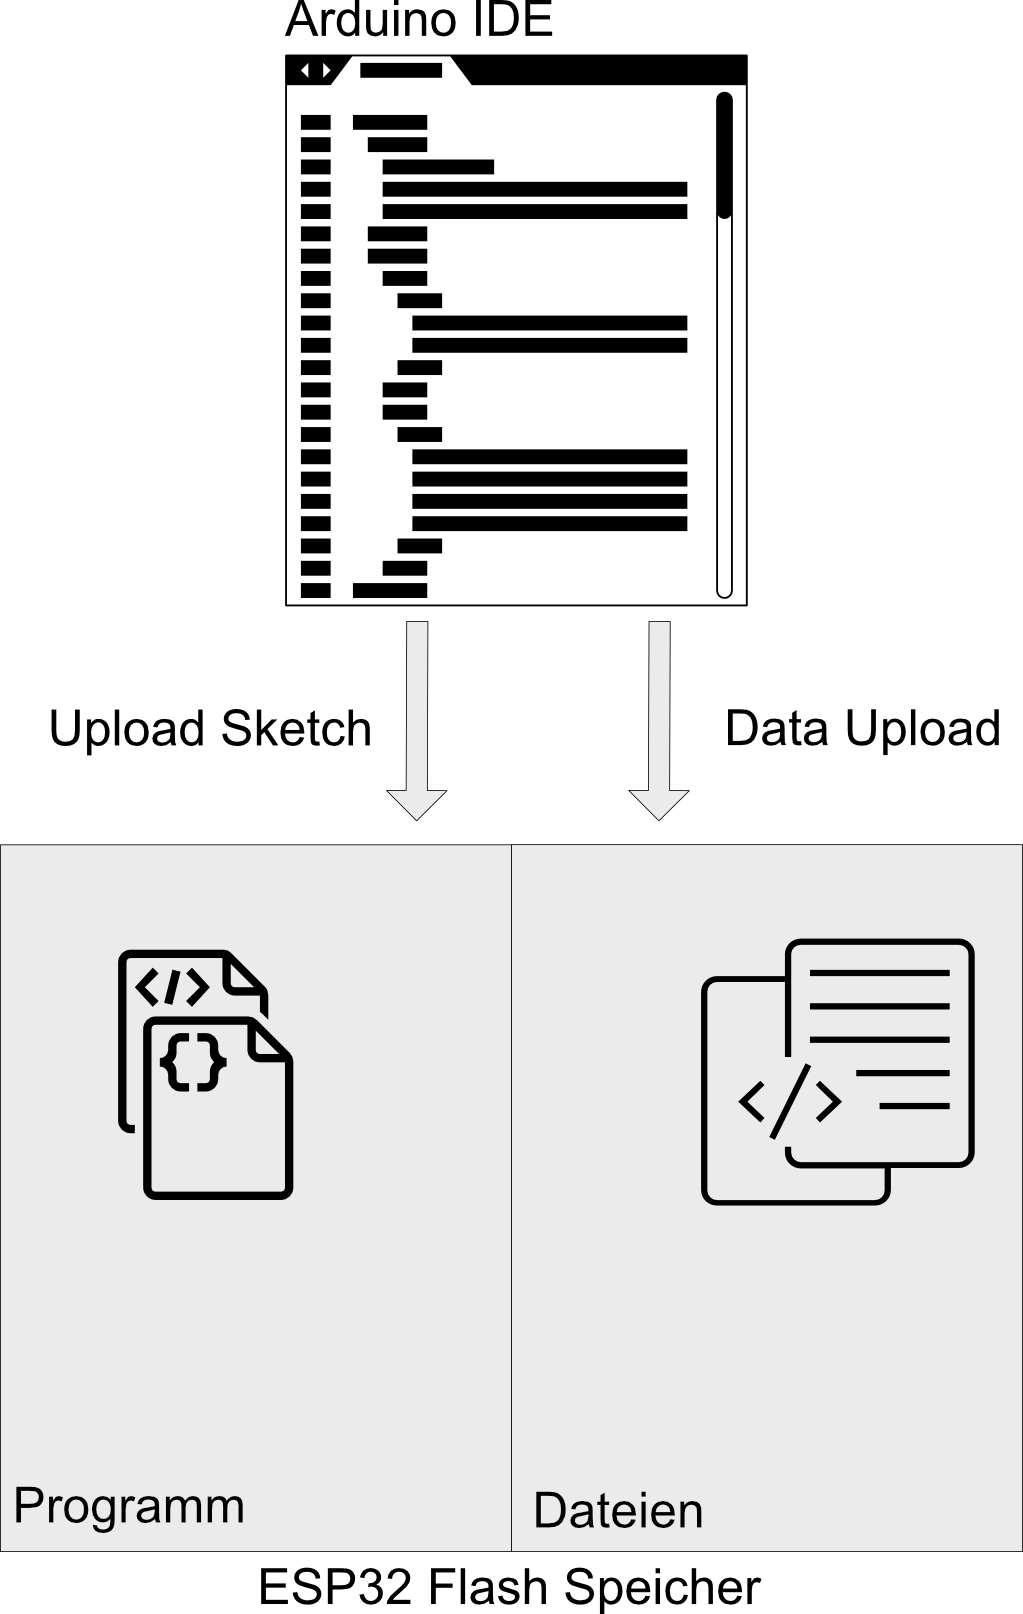
\includegraphics[width=7cm, left]{Bilder/ESP32-Memory-Organisation.png}}
    \captionsetup{justification=centering}
    \captionof{figure}{Speicher-Aufteilung ESP32}
	\end{minipage}
\end{center}

 Jeder Sensor benötigt einige Parameter:
 \begin{description}
\item[Id] Identifiziert den Sensor, gespeichert in der Datei id.txt
\item[key] Der geheime Schlüssel um den \Gls{hmac} zu berechnen, gespeichert in der Datei key. Dieser Schlüssel muss auf den Sensoren wie auf dem Gateway identisch sein.
\end{description}
Die folgende Parameter werden alle in der Datei settings.txt gespeichert:
 \begin{description}
\item[sensorType] Typ des Temperatursensor, entweder DHT11 oder DHT22
\item[sleepTime] Wartezeit zwischen zwei Messungen in Millisekunden
\item[paLevel] Funkstärke des NRF24 Moduls, erlaubte Werte sind 'low', 'med und 'high'
\end{description}

\subsection{Datenübertragung}Durch die Verwendung des \Gls{hmac} wird die Nachricht stark vergrössert und erreicht um die neunzig Zeichen.
Da die maximale Grösse eines Datenpaketes des NRF24 Moduls nur 32 Zeichen beträgt, muss die gesamte Nachricht in mehreren Paketen übertragen werden.

\begin{center}
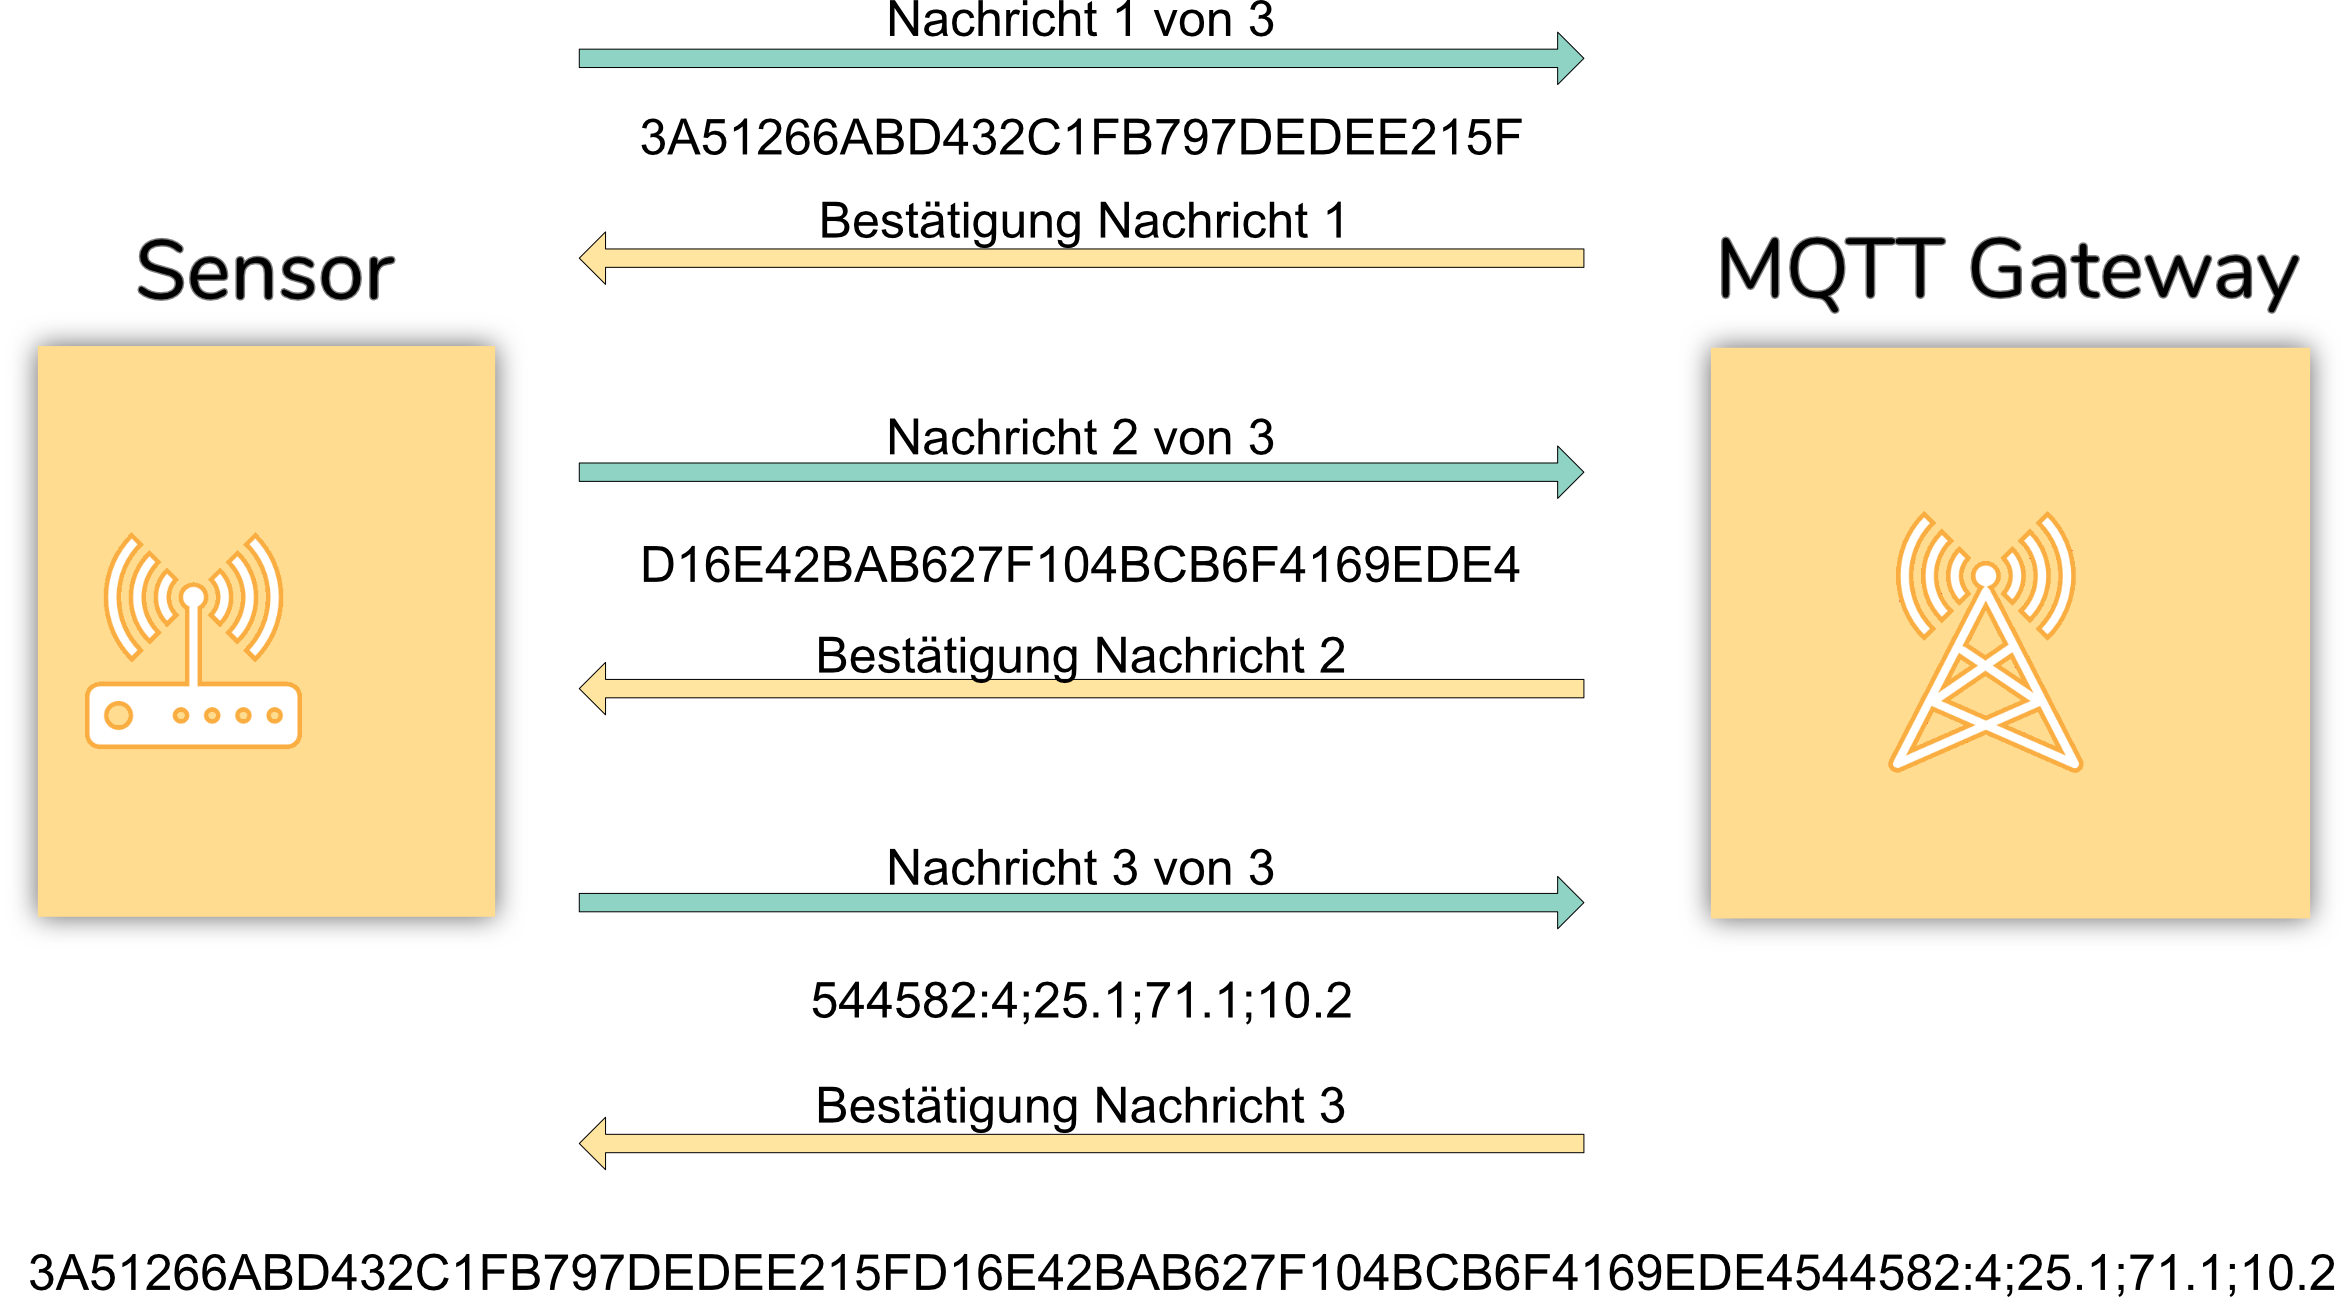
\includegraphics[width=17cm, left]{Bilder/Funkprotokoll.png}
 \captionsetup{justification=centering}
\captionof{figure}{Übertragen der Messdaten in mehreren Paketen}\label{radioprotocol}
\end{center}
\begin{minted}{arduino}
bool ok = radio->write( &sending, sizeof(sending));    //Sends first packet to radio

if (ok) {
  byte packetReceived = 0;  //packetReceived (feedback) = 0th packet
  radio->startListening();    //start listening for a response
  int retry = 0;
  while (!confirmed && retry < 5) {
    delay(50);
    if (radio->available()) {
      radio->read(&packetReceived, sizeof(packetReceived));    //save response
      if (packetReceived == pkt) {  //If packet number received == packet sent
        confirmed = true;
        Serial.println("Packet was confirmed, proceed to send next packet.");
      }
      else {
        confirmed = false;
        sendArray = false;
        Serial.println("Either nothing sent/no confirmation/Mismatch of packets (resend??)");
      }
    }
    retry++;
  }
  radio->stopListening();
}
\end{minted}
\chapter{MQTT Gateway}
\section{Übersicht}
\begin{center}
    \begin{minipage}[t]{0.3\textwidth}
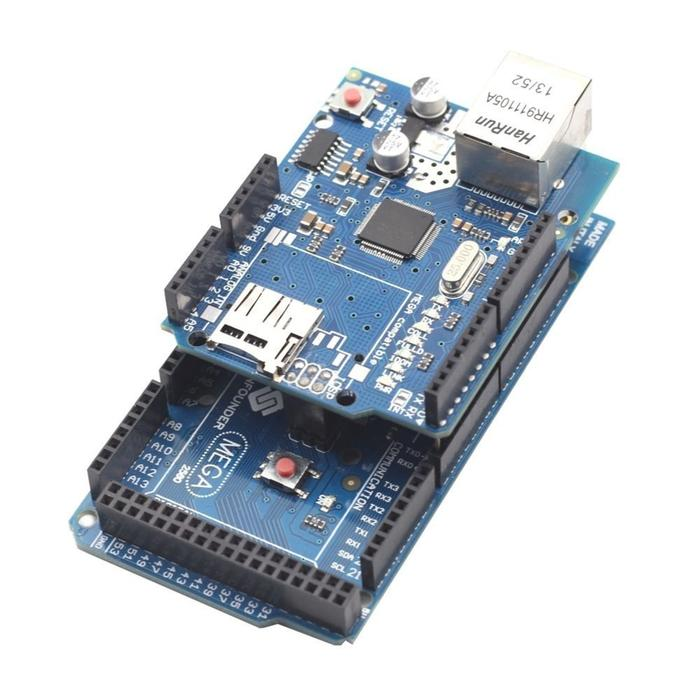
\includegraphics[width=5cm, left, valign=t]{Bilder/ArduinoWithEthernetShield.jpg}
	\end{minipage}\hfill
    \begin{minipage}[t]{0.7\textwidth}
    Die Aufgabe des \Gls{mqtt} Gateways ist es die Messdaten, welche über Funk gesendet werden, zu empfangen und an den \Gls{mqtt} Broker weiterzuleiten. Dazu ist es mit einem Funkmodul und einer Ethernet Schnittstelle ausgerüstet.
    \end{minipage}
\end{center}

\section{Hardware}
Die Basis des MQTT Gateway bildet ein Arduino Mega [\ref{arduino}] welcher mit einem Ethernet Shield kombiniert wird. Die Funkverbindung wird wie bei den Sensoren durch ein NRF24 [\ref{nrf24}] Modul hergestellt.
\subsection{Aufbau}
Die Stromversorgung des Funkmoduls erfolgt über VCC (3.3V) und GND. 

Die zusätzlichen Pins werden wie folgt mit dem Arduino verbunden (Links -> Pin Arduino, Rechts -> Anschluss Funkmodul):
\begin{itemize}[noitemsep,topsep=0pt,parsep=0pt,partopsep=0pt]
\item 8 - CSN
\item 7 - CD
\item 52 - SCK
\item 51 -  MOSI
\item 50 - MISO
\end{itemize}
\begin{center}
    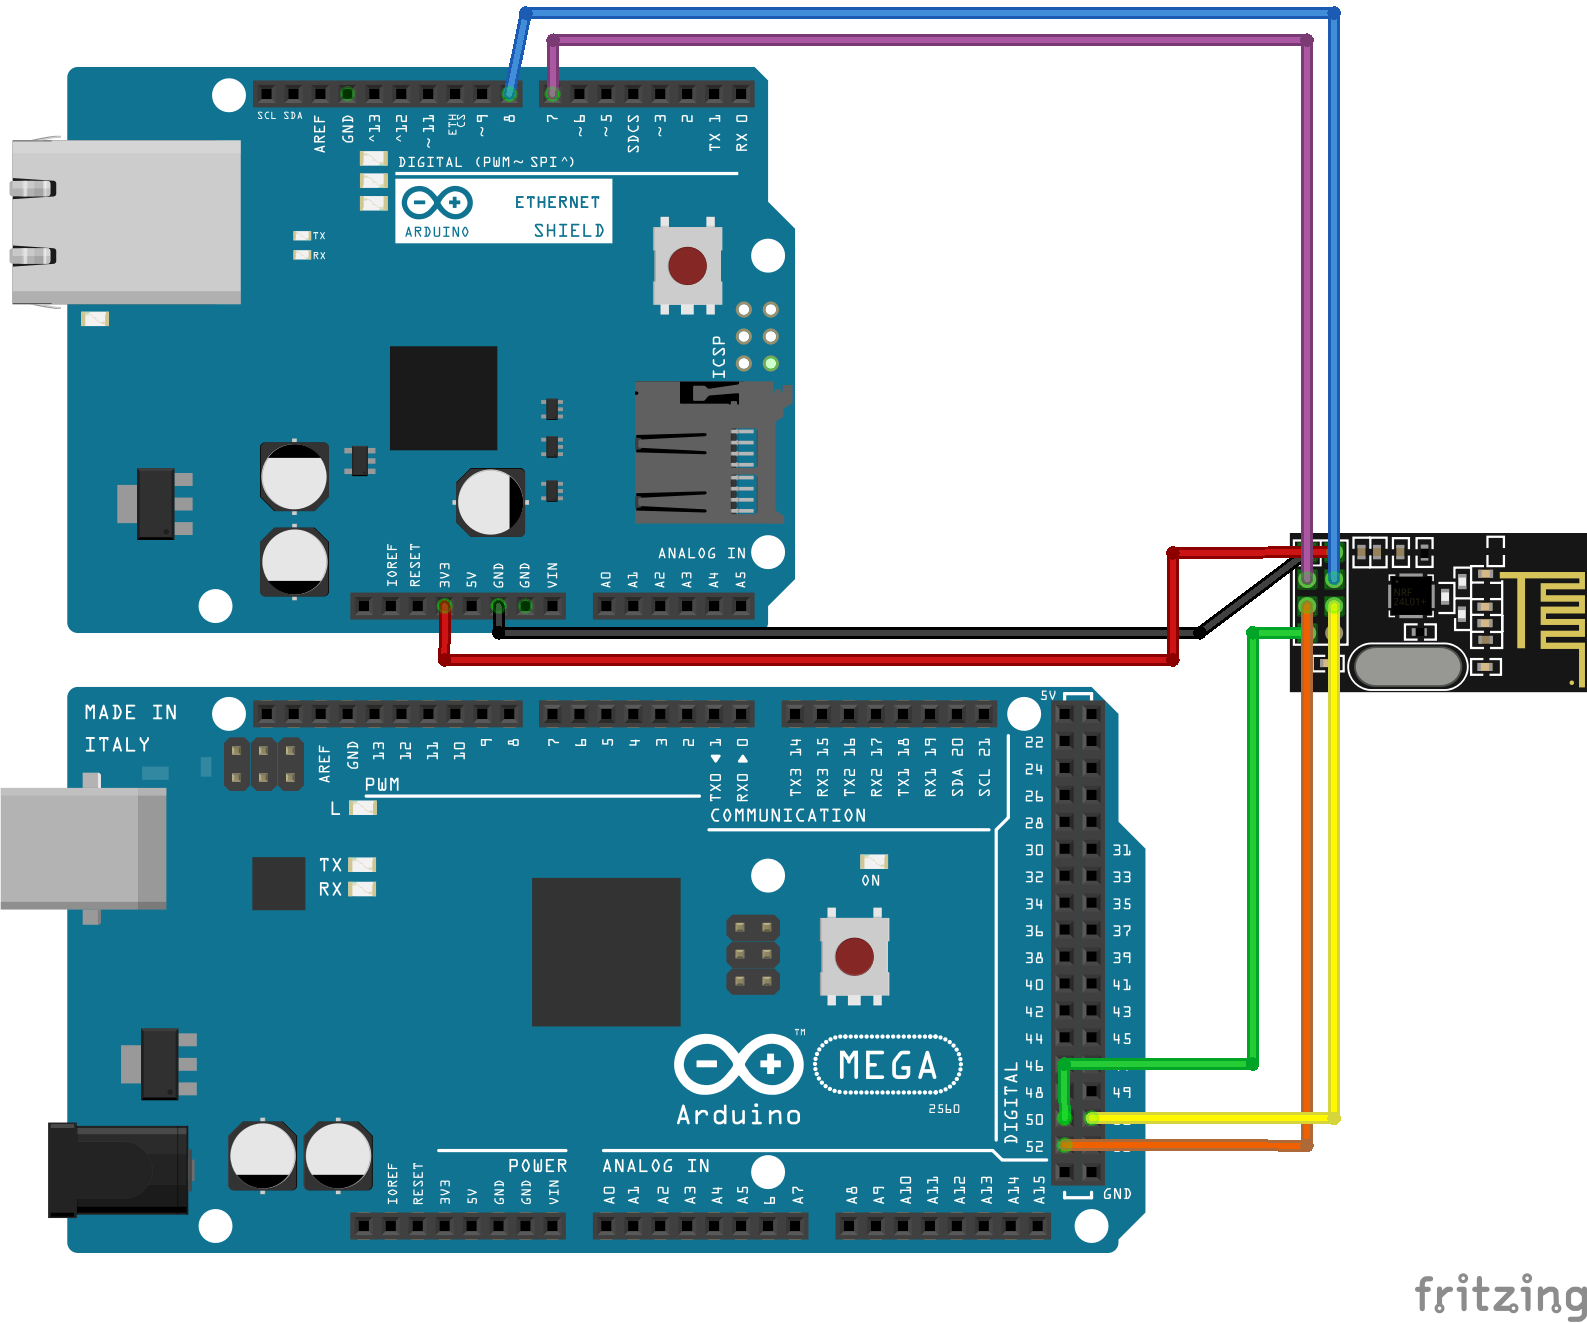
\includegraphics[width=12cm, left]{Bilder/MQTT-Gateway-Design_Steckplatine.png}
    \captionof{figure}{Verdrahtung der Komponenten}
\end{center}
\subsection{Zugriffsschutz}
Jede empfangene Nachricht wird durch die Valdierung des HMAC (\Gls{hmac}) sowohl auf einen berechtigten Absender, als auch auf unverfälschte Daten überprüft [\ref{funkAbsicherung}].

Der Empfänger der Nachricht, welcher denselben geheimen Schlüssel wie der Sender verwendet, berechnet aus den übertragenen Daten ebenfalls den \Gls{hmac} und vergleicht den selbst berechneten Wert mit dem empfangenen Wert. Wenn diese beiden Werte nicht übereinstimmen so wird der Datensatz verworfen.
\subsection{Warum kein TLS?}
Die etablierten Verschlüsselungstechniken wie Transport Layer Security (oder SSL) können mit \Gls{iot} Geräten nicht verwendet werden. Ein Verbindungsaufbau mit TLS ist ein Zeit- und Rechenintensiver Prozess welcher ein vielfaches der Übertragungsdauer der Daten in Anspruch nehmen würde. Der Stromverbrauch wäre mit einer solchen Technik hoch und die Laufzeiten der Geräte zu gering.
\section{Software}
 \subsection{Verwendete Bibliotheken}

  \begin{description}
\item[pubsubclient] Anbindung eines MQTT Brokers \cite{pubsubclient}
\item[ethernet] Benutzung einer Ethernet Verbindung \cite{ethernet}
\item[NRF24] Verwendung des NRF24 Funkmoduls \cite{nrf24Arduino}
\item[cryptosuite] SHA und HMAC Berechnungen \cite{cryptosuite}
 \end{description}
 \subsection{Empfang der Daten}
 Um von allen Sensoren Daten empfangen zu können wird auf jeder Adresse eines Sensors ein Kanal geöffnet.
 \begin{minted}{arduino}
  Serial.println(F("Open pipes"));
  for (int i = 1; i < pipes_length; i++) {
    radio.openReadingPipe(i, pipes[i]);
    Serial.print(F("Listening to pipe: "));
    char c_address[8];
    sprintf(c_address, "-> %s", pipes[i]);
    Serial.print(c_address);
    Serial.print(" on channel ");
    Serial.println(i);
  }
 \end{minted}
 Sobald ein Paket empfangen wird, extrahiert das Gateway die Anzahl Pakete pro Nachricht und fordert das nächste fehlende Paket vom Sensor an.
 \begin{minted}{arduino}
 byte data[32];
      if (!allReceived && radio.available()) {
        radio.read( &data, sizeof(data) );//place received data in byte structure
        byte pkt = data[0];  //part of header, packet number received

        for (int i = 2; i < 32; i++) {
          received[(pkt - 1) * 30 + (i - 2)] = data[i];
        }
        delay(5);
        radio.stopListening();    //stop listening to transmit response of packet received.

        byte* address = pipes[pipe_num];
        radio.openWritingPipe(address);
        bool ok = radio.write(&pkt, sizeof(pkt));  //send packet number back to confirm
\end{minted}
Sobald die gesamte Nachricht empfangen wurde wird der \Gls{hmac} mit dem durch das Gateway selbst berechneten Wert verglichen:
\begin{minted}{arduino}
char* hmac = strtok(received, ":");
char* data = strtok(NULL, ":");

Sha256.initHmac(key, keyLength);
Sha256.print(data);
 uint8_t* calculatedHmac = Sha256.resultHmac();

char calculatedHmac_char[hmacSize * 2];
for (int cnt = 0; cnt < hmacSize; cnt++)
{
   // convert byte to its ascii representation
    sprintf(&calculatedHmac_char[cnt * 2], "%02X", calculatedHmac[cnt]);
 }

uint8_t authorizationCheck = strcmp(calculatedHmac_char, hmac);

 if (authorizationCheck != 0) {
   Serial.println("Hmac not matching, not authorized or tampered message! Message rejected");
 }
\end{minted}
Falls der empfangene Wert und der berechnete Wert nicht übereinstimmen wird die Nachricht verworfen.
 \subsection{Senden der Daten an den MQTT Broker}
Nachdem die Nachricht eines Sensors validiert wurde, wird das Format in JSON umgewandelt und an ein MQTT Topic verschickt.
\begin{center}
	\begin{minted}{js}
	{     
	    "ID": 0001, 
	    "Temp.Air": 22.6,
	    "Hum.Air": 78.1, 
	    "Hum.Soil": 43.7
	}
	\end{minted}
	\captionof{figure}{Sensor Datensatz in JSON Format} 
	\label{json-example}
\end{center}
Alle Datensätze werden in ein gemeinsames Topic namens "/weather/" gespeichert. In einer frühen Version hatte ich für jede Kategorie von Messwerten (Lufttemperatur, Luftfeuchtigkeit etc.) ein eigenes Topic verwendet.  Dies war aber unpraktisch für die Weiterverarbeitung und wurde zu einem einzelnen Topic geändert.
\begin{center}
	\begin{minted}{arduino}
char json[100];
sprintf(json, "{\"ID\": \"%s\", \"Temp.Air\": %s, \"Hum.Air\": %s, \"Hum.Soil\": %s}", SensorId, Temperature, Humidity, SoilHumidity);
if (!client.connected()) {
  reconnect();
}
if (client.connected()) {
  Serial.print("Send data to topic '/weather/' ");
  client.publish("/weather/", json);
  Serial.println(json);
}
\end{minted}
\end{center}

\subsection{Konfiguration}
Das Gateway benötigt für die Berechnung des \Gls{hmac} den gleichen Schlüssel wie der Sensor. Leider bietet der Arduino nicht die Möglichkeit Dateien in einem eigenen Speicherbereich abzulegen. Der benötigte geheime Schlüssel wird deshalb in der Datei keyFile.h als String definiert. So kann der Code weiterhin in dem Versionskontrollsystem hinterlegt werden ohne den geheimen Schlüssel preisgeben zu müssen.
\begin{center}
    \begin{minipage}[b]{0.4\textwidth}
    	Die Datei keyFile.h enthält nur eine Zeile mit der Deklaration des Schlüssels \mint{html}|String key_str  = "geheimerSchlüssel";|
    \end{minipage}\hfill
    \begin{minipage}[b]{0.4\textwidth}
	\begin{forest}
		    for tree={font=\sffamily, grow'=0,
		    folder indent=.9em, folder icons,
		    edge=densely dotted}
	       [Arduino{\_}NRF24{\_}Receiver
		    	[Arduino{\_}NRF24{\_}Receiver.ino, is file]
		    	[keyFile.h, is file]
		    ]
	\end{forest}
	\end{minipage}
\end{center}

\chapter{Speicherung und Visualisierung}
\section{Übersicht}
Für die Speicherung und Verarbeitung der gesammelten Sensordaten sind mehrere Softwarekomponenten zuständig.
\begin{center}
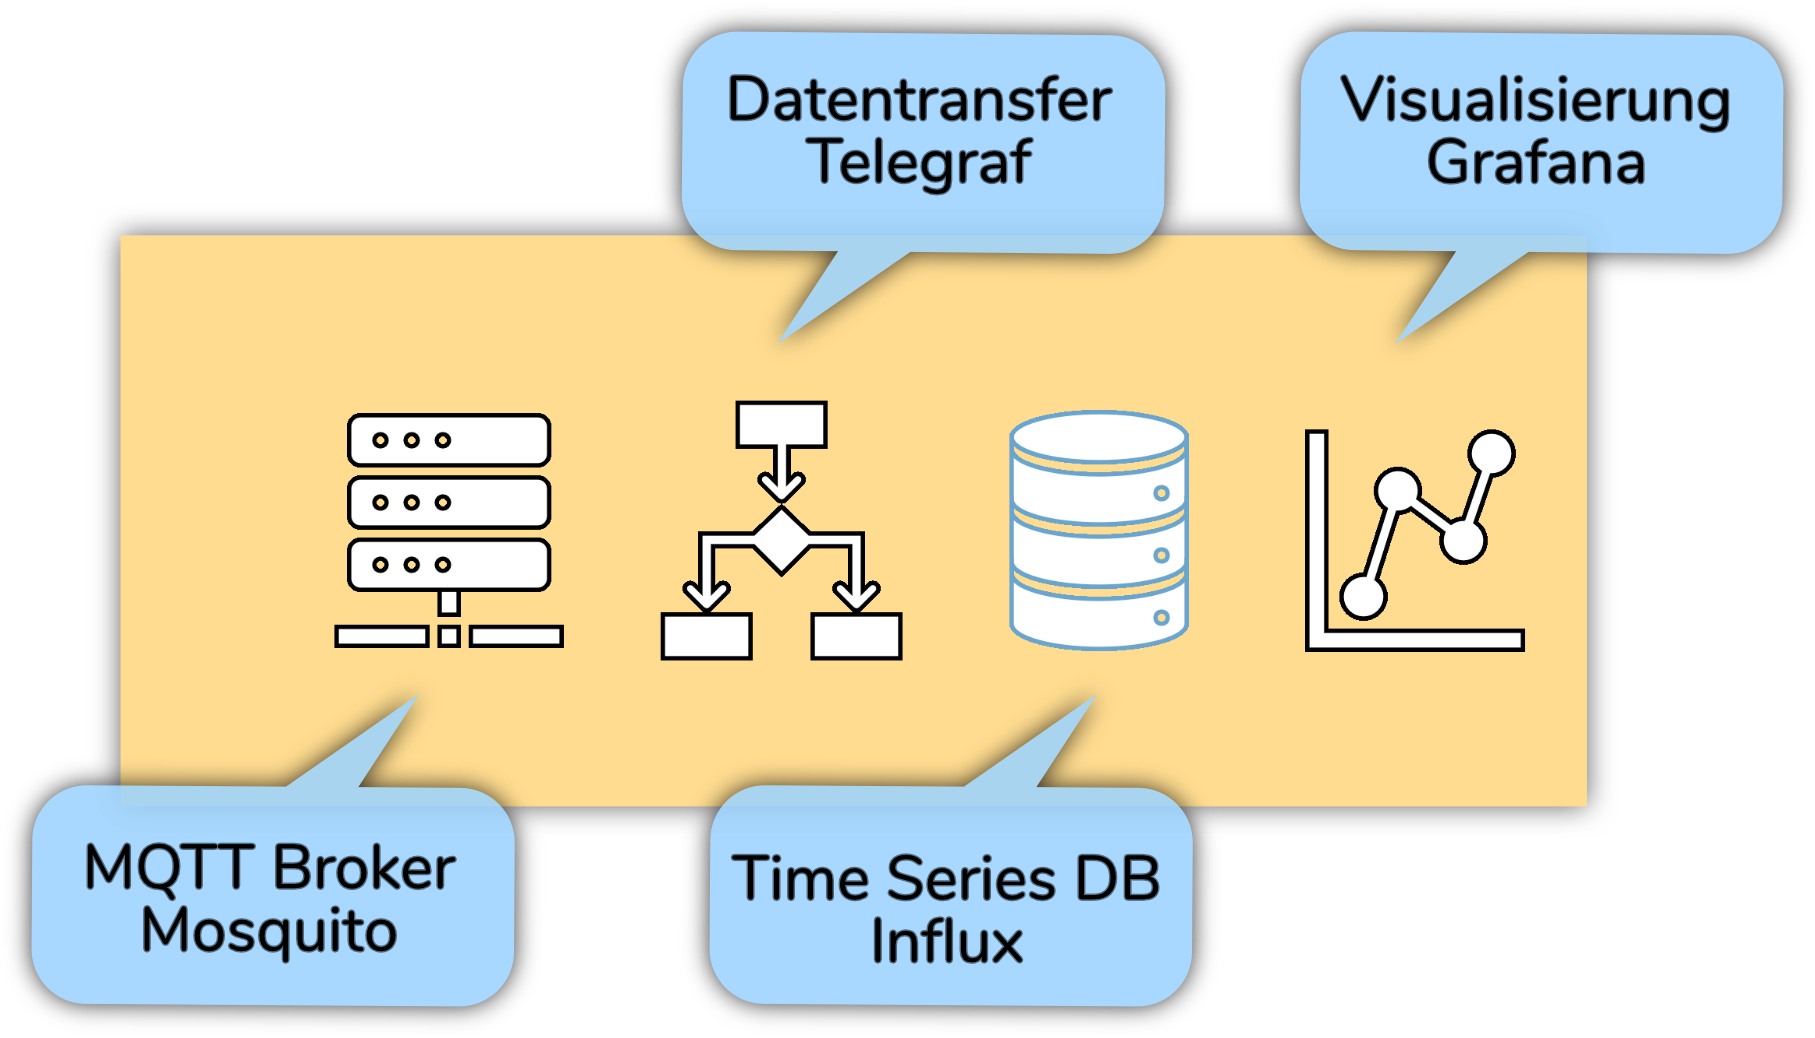
\includegraphics[width=17cm, left]{Bilder/Raspberry-Software.png}%
\captionof{figure}{Verwendete Software}\label{labelname}%
\end{center}
 \begin{description}
\item[MQTT Broker] Die von dem MQTT-Gateway geschickten Nachrichten werden durch Mosquitto \cite{mosquitto} in einer Queue bis zu einer weiteren Verarbeitung gespeichert
\item[Datentransfer] Um die Daten aus einer (oder mehreren) MQTT Queue in eine Datenbank zu transferieren wird Telegraf \cite{telegraf} mit dem MQTT Plugin benutzt \cite{telegrafmqtt}
\end{description}
\section{Hardware}
Als Plattform für Mosquitto \cite{mosquitto}, Telegraf \cite{telegraf}, InfluxDB \cite{influx} und Grafana \cite{grafana} dient ein Raspberry Pi2 Model B [\ref{raspberry}].
\section{MQTT Broker}
Als MQTT Broker wird die Open Source Software Mosquitto \cite{mosquitto} verwendet.
\subsection{Installation}
Die Installation von Mosquitto sollte ebenfalls den Mosquitto-Client umfassen, damit man nach der Installation diese direkt testen kann.
\begin{minted}{shell}
sudo apt-get install -y mosquitto mosquitto-clients
   \end{minted}
 Um den Broker automatisch bei jedem Neustart zu starten, muss der Service noch aktiviert werden.
 \begin{minted}{shell}
systemctl enable mosquitto.service
 \end{minted}
 
 \subsection{Warum kein TLS?}
Eigentlich wollte ich SSL mit Client-Zertifikaten für die Verbindung zwischen dem MQTT Gateway und dem MQTT Broker verwenden. Beispiele dazu kann man im Internet finden, sogar eine direkte Verbindung zwischen ESP32 Geräten und einem MQTT Broker mit SSL Mutual Auth ist möglich [\cite{espssl}, \cite{mosquittoSSL}].

Allerdings stellte sich heraus, dass die Ethernet Bibliothek kein SSL unterstützt. Die WI-FI Bibliothek unterstützt dies hingegen und es gibt Tips wie man mit einigen Klassen aus der WI-FI Implementierung die Ethernet Bibliothek anpassen könnte. Ich habe allerdings aus Zeitgründen dieses Thema nicht weiter verfolgt.
\section{Datenspeicherung}
Die Messdaten werden in der Zeitreihendatenbank Influx \cite{influx} gespeichert. Eine Zeitreihendatenbank erlaubt das schnelle schreiben von Messwerten und kann automatisch ältere Datensätze entfernen um den Platzbedarf nicht zu gross werden zu lassen.
  \begin{center}
    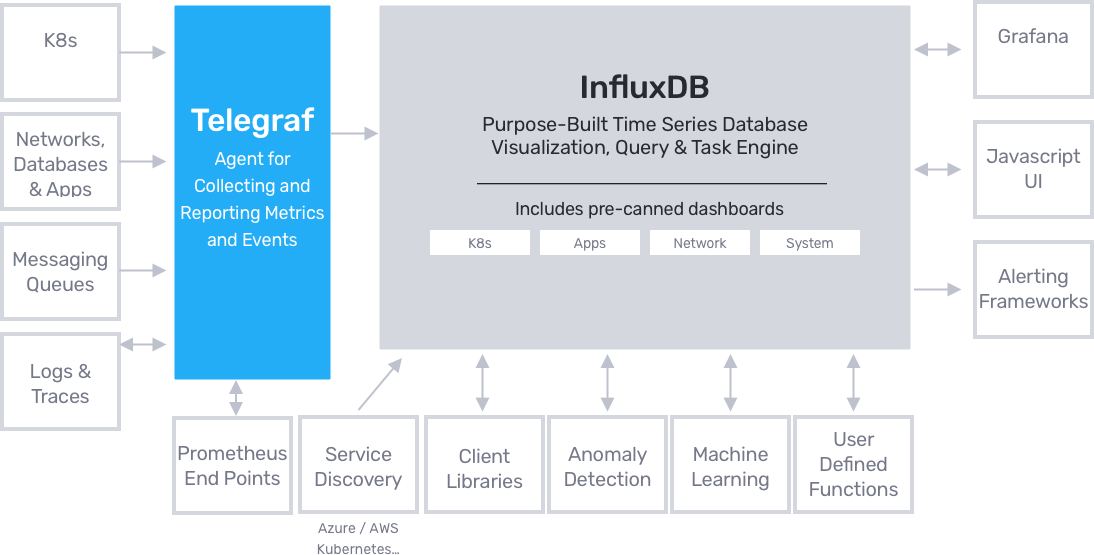
\includegraphics[width=\textwidth, valign=t]{Bilder/InfluxDB-2.png}
    \captionsetup{justification=centering}
    \captionof{figure}{Übersicht Influx Software}
    \source{\url{www.influxdata.com}}
   \end{center}
   \subsection{Telegraf}
Um die Daten aus dem MQTT Topic zu lesen und in die Datenbank zu schreiben, wird die Software Telegraf \cite{telegraf} eingesetzt.
\subsubsection{Installation / Konfiguration}
Telegraf wird zusammen mit InfluxDB installiert und muss nur noch konfiguriert werden. Eine Konfigurationsdatei kann initial mit dem Kommando \mint[breaklines=true]{shell}|telegraf -sample-config -input-filter mqtt_consumer -output-filter influxdb > telegraf.conf| erzeugt werden.

In der erzeugten Datei muss das Einlesen der MQTT Queue im Abschnitt ''[[inputs.mqtt{\_}consumer]]'' angepasst werden.
\begin{minted}{shell}
[[inputs.mqtt_consumer]]
   servers = ["tcp://localhost:1883"]
   topics = [
     "/weather/",
   ]
    topic_tag = "weather"
    qos = 0
    connection_timeout = "30s"
    max_undelivered_messages = 1000
    client_id = "telegraf"
    data_format = "json"
    tag_keys = ["ID"]
\end{minted}
Auch das Schreiben der Daten in die Influx Datenbank muss im Abschnitt ''[[outputs.influxdb]]'' konfiguriert werden.
\begin{minted}{shell}
[[outputs.influxdb]]
  urls = ["http://localhost:8086"]
  database = "weather_db"
  timeout = "5s"
  username = "telegraf"
  password = "***************"
  user_agent = "telegraf"
\end{minted}

Zuletzt wird Telegraf mitgeteilt welche Konfigurationsdatei verwendet werden soll: \mint{shell}|telegraf --config telegraf.conf|
\subsection{InfluxDB}
   \subsubsection{Installation}
   Die Installationsquelle ist unterschiedlich für die verschiedenen Linux Distributionen. Wenn, wie in meinem Fall, die Raspian Distribution in der Version 'buster' verwendet wird, kann das benötigte Repository mit folgenden Kommandos hinzugefügt werden:
 \begin{minted}[breaklines]{shell}
curl -sL https://repos.influxdata.com/influxdb.key | sudo apt-key add -
sudo apt install apt-transport-https
echo "deb https://repos.influxdata.com/debian buster stable" | sudo tee /etc/apt/sources.list.d/influxdb.list
\end{minted}
Die Installation ist schnell gemacht:
 \begin{minted}{shell}
sudo apt-get update && sudo apt-get install influxdb
sudo systemctl unmask influxdb.service
   \end{minted}
   Anschliessend muss der Service noch gestartet werden:
    \begin{minted}{shell}
sudo systemctl start influxdb
   \end{minted}
   \subsubsection{Datenbank einrichten}
{\color{red}Achtung: Standardmässig ist die Influx Datenbank ohne Authentifizierung eingerichtet. In einem offenen Umfeld sollte die standardmässige Authentifizierung eingeschaltet werden \cite{influxAuth}}

Um eine Datenbank und einen Benutzer einzurichten verwendet man das Kommondozeilen-Tool \mint{shell}|influx|
 \begin{minted}{shell}
Connected to http://localhost:8086 version 1.7.7
InfluxDB shell version: 1.7.7
> CREATE DATABASE weather_db
> USE weather_db
 >CREATE USER telegraf WITH PASSWORD '*******************'
 >GRANT [READ,WRITE,ALL] ON weather_db TO telegraf
 \end{minted}
 Eine Spaltendefinition ist nicht nötig, die Spalten werden direkt aus den empfangenen Daten gebildet.
\section{Visualisierung}
Die Visualisierung der Daten wird über die Open Source Software Grafana \cite{grafana} durchgeführt. Mit dieser Software können nicht nur Zeitreihen dargestellt werden, es ist auch möglich bei der Überschreitung von Schwellwerten Alarm auszulösen.
\subsection{Installation}
Grafana für den Raspberry Pi kann nicht über ein Repository installiert werden, weshalb die aktuelle Version zuerst mit \mint{shell}|wget| heruntergeladen und danach entpackt wird.
 \begin{minted}[breaklines]{shell}
wget https://github.com/fg2it/grafana-on-raspberry/releases/download/v5.1.4/grafana_5.1.4_armhf.deb
sudo apt-get install -y adduser libfontconfig1
sudo dpkg -i grafana_5.1.4_armhf.deb
sudo systemctl enable grafana-server
sudo systemctl start grafana-server
sudo systemctl enable grafana-server.service
   \end{minted}
   \subsection{Grafana Dashboard}
Die Darstellung der Messwerte erfolgt in Grafana über Panels, welche in einem Dashboard \cite{grafanaDashboard} zusammengefasst werden.
\begin{center}
   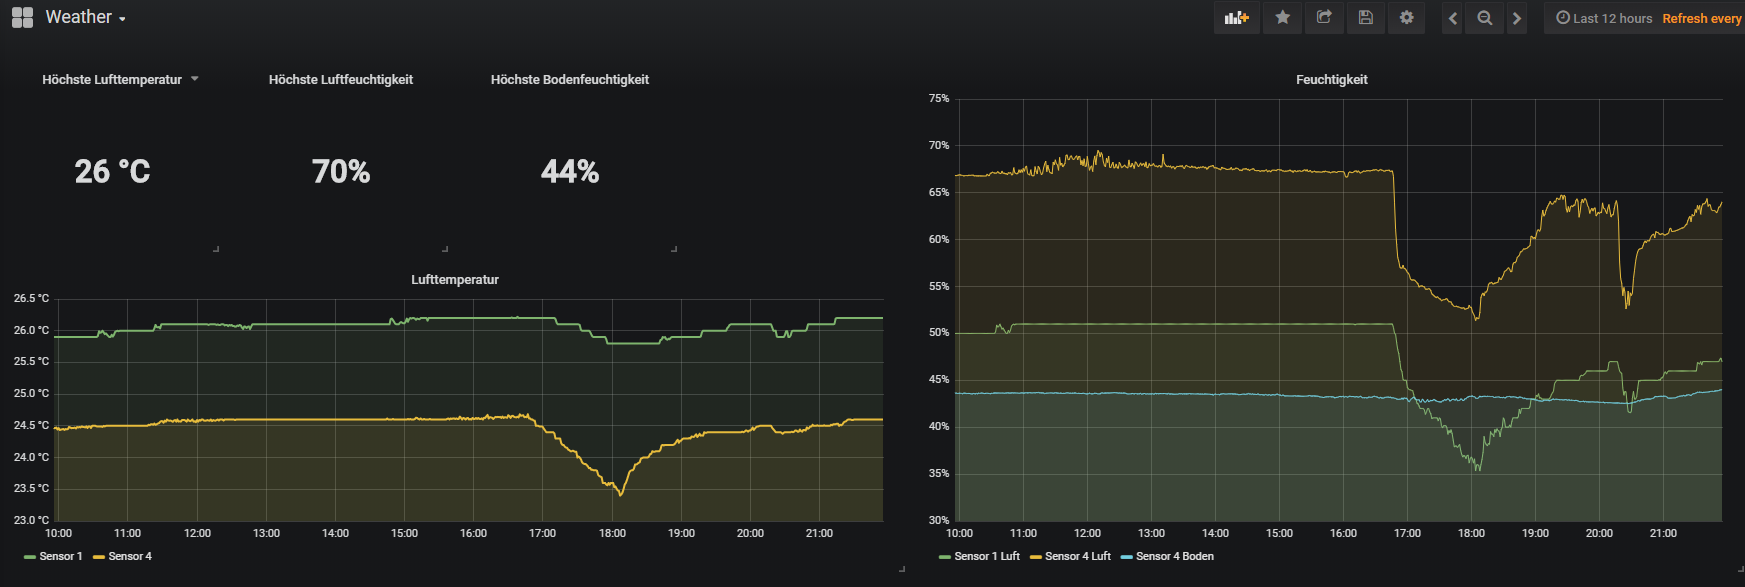
\includegraphics[width=17cm]{Bilder/Grafana-Dashboard.PNG}
   \captionsetup{justification=centering}
    \captionof{figure}{Grafana Dashboard}
\end{center}

\begin{center}
    \begin{minipage}[t]{0.45\textwidth}
        \centering
        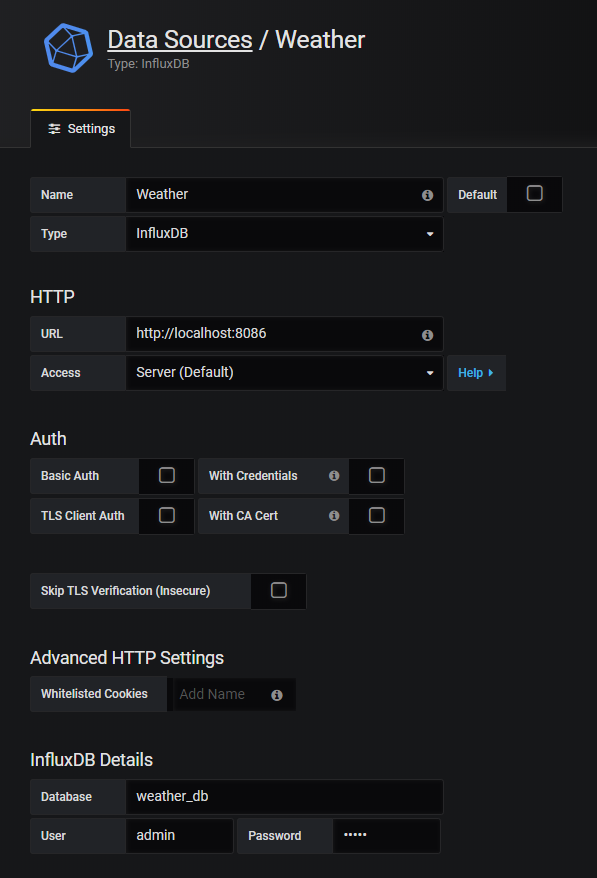
\includegraphics[width=5cm, valign=t]{Bilder/Grafana-Datasource.PNG} % first figure itself
        \captionsetup{justification=centering}
        \captionof{figure}{Grafana: Konfiguration Influx Datenquelle}
    \end{minipage}
    \begin{minipage}[t]{0.45\textwidth}
Bevor ein Dashboard erstellt wird, muss man die Datenquellen definieren. Hier ist die Konfiguration der Datenquelle, welche aus der lokal installierten InfluxDB und der Datenbank weather{\_}db die Messwerte liest.
    \end{minipage}
\end{center}

\begin{center}
    \begin{minipage}[t]{0.45\textwidth}
        \centering
        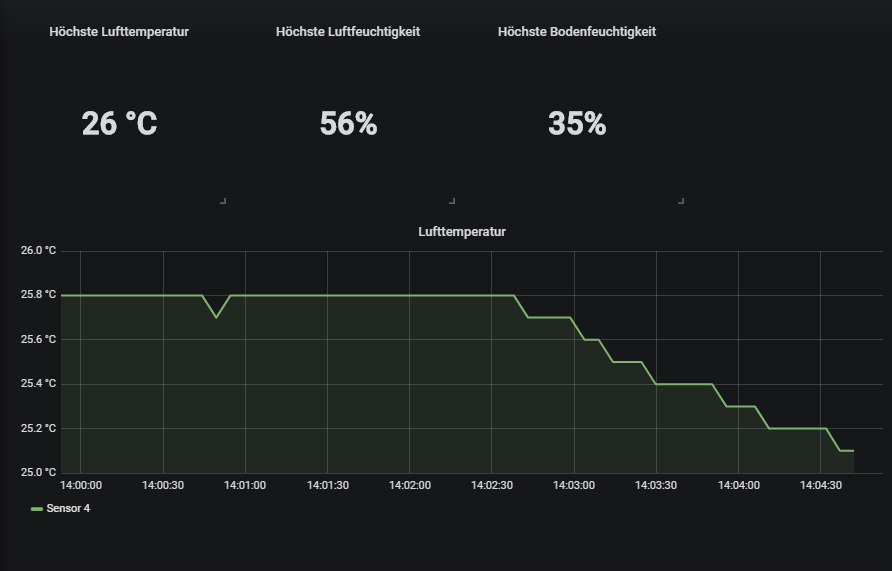
\includegraphics[width=7cm, valign=t]{Bilder/Grafana-Luft.PNG} % first figure itself
        \captionsetup{justification=centering}
        \captionof{figure}{Grafana Dashboard: Panel Lufttemperatur}
        
        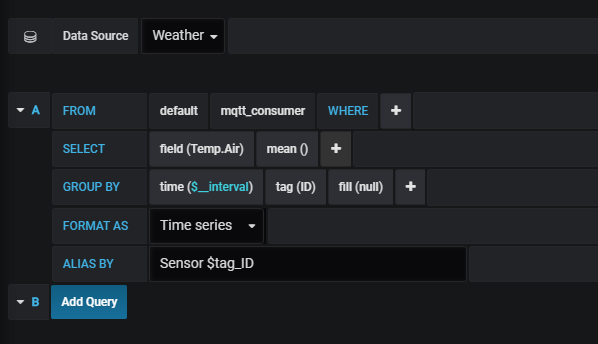
\includegraphics[width=7cm, valign=t]{Bilder/Grafana-Panel-Konfiguration.PNG}
        
         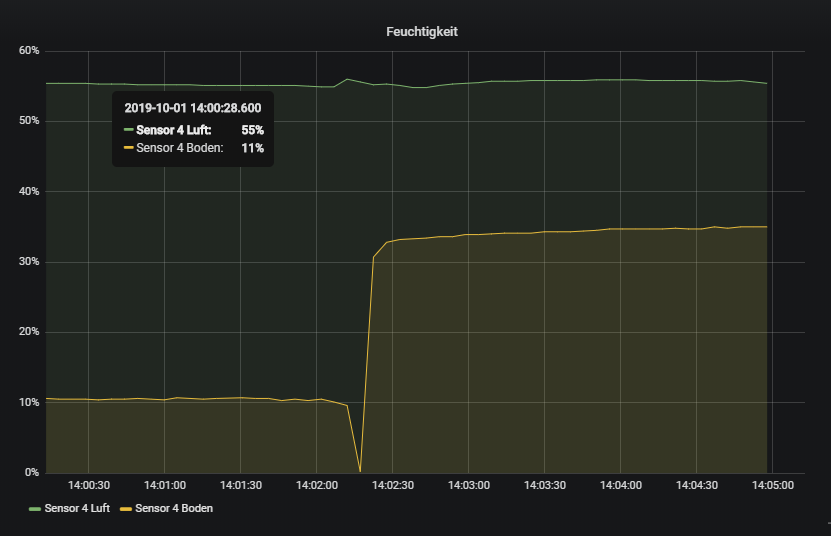
\includegraphics[width=7cm, valign=t]{Bilder/Grafana-Feuchtigkeit.png} % second figure itself
        \captionsetup{justification=centering}
        \captionof{figure}{Grafana Dashboard: Panel Feuchtigkeit}
    \end{minipage}
    \begin{minipage}[t]{0.45\textwidth}
Die Datenbankabfrage für jedes Panel kann direkt in der Benutzeroberfläche von Grafana erstellt werden. Dabei können die Mittelwerte über mehrere Messwerte gebildet werden oder auch nur der maximale Wert in einem bestimmten Zeitintervall bestimmt werden. In dem Weather Dashboard werden von allen drei Mess-Kategorien die höchsten Werte der letzten Tage dargestellt neben den Panels mit dem zeitlichen Verlauf.
\break
\break
Die Legende wird normalerweise aus den Werten der Datenquelle und der Zeitreihe gebildet, was sehr unverständlich sein kann. In der Konfiguration eines Panels kann deshalb im Feld ''ALIAS BY'' eine alternative Bezeichnung angegeben werden. In diesem Beispiel ist es \mint{js}|Sensor $tag_ID| was dazu führt, dass jeweils der Text ''Sensor'' und die Id des Sensors verwendet wird.
    \end{minipage}
\end{center}
\section{Ersatz für Kafka}
Ursprünglich war geplant zwischen dem MQTT Broker und InfluxDB den Apache Kafka Message Bus mit Streams zu verwenden. Die Installation von Zookeper und Kafka auf dem Raspberry Pi verlief problemlos und die Software lies sich starten und testen. Um die Nachrichten aus dem MQTT Topic zu lesen und in ein Kafka Topic zu schreiben kann man das Kafka Connect Framework mit dem Kafka Connect MQTT Connector verwenden \cite{connect}. Allerdings ist der MQTT Connector nicht frei verfügbar (im Gegensatz zu Kafka selber) und kann kostenlos nur mit einer 30 Tage Testlizenz betrieben werden. Zudem erwies sich Kafka Connect als sehr Resourcen intensiv. In der Default Einstellung wird von 2GB Ram alleine für Kafka Connect ausgegangen. Da der Raspberry Pi nur 1GB Ram besitzt musste ich diesen Wert reduzieren. Der Connector lies sich danach starten, es dauert aber sehr lange bis der MQTT Adapter bereit war. Aufgrund dieser Erfahrungen habe ich nach alternativen gesucht und bin dabei bei Telegraf gelandet. Meine Erfahrungen damit sind ausgesprochen positiv, der Speicherbedarf ist viel geringer und die Geschwindigkeit höher. 

Anstatt den MQTT Connector zu verwenden wäre es natürlich auch mit einem eigenen Programm oder Skript möglich gewesen die Nachrichten aus dem MQTT Broker zu lesen und in ein Kafka Topic zu schreiben. Dies hätte jedoch Zeit des Projektes verbraucht welche ich lieber für andere Punkte aufwenden wollte.
{\let\clearpage\relax \chapter{Fazit}}
Die in diesem CAS behandelten Komponenten Mosquitto und Influx können sehr gut für \Gls{iot} Projekte eingesetzt werden. Insbesondere die gute Performance auf der sehr schwachen Hardware in diesem Projekt (Raspberry Pi 2)  war überraschend. Als negative Erfahrung gilt für mich Kafka Connect und insbesondere der MQTT Connector. Nicht nur die Installation war mühsam, auch die Geschwindigkeit lag nicht im akzeptablen Bereich. Der Unterschied zwischen dem in Go geschriebenen Telegraf und der Java Applikation Kafka Connect war massiv.
{\let\clearpage\relax \chapter{Verwendete Bauteile}}
\section{ESP32 Mikrokontroller}
\begin{minipage}[t]{0.5\linewidth}
	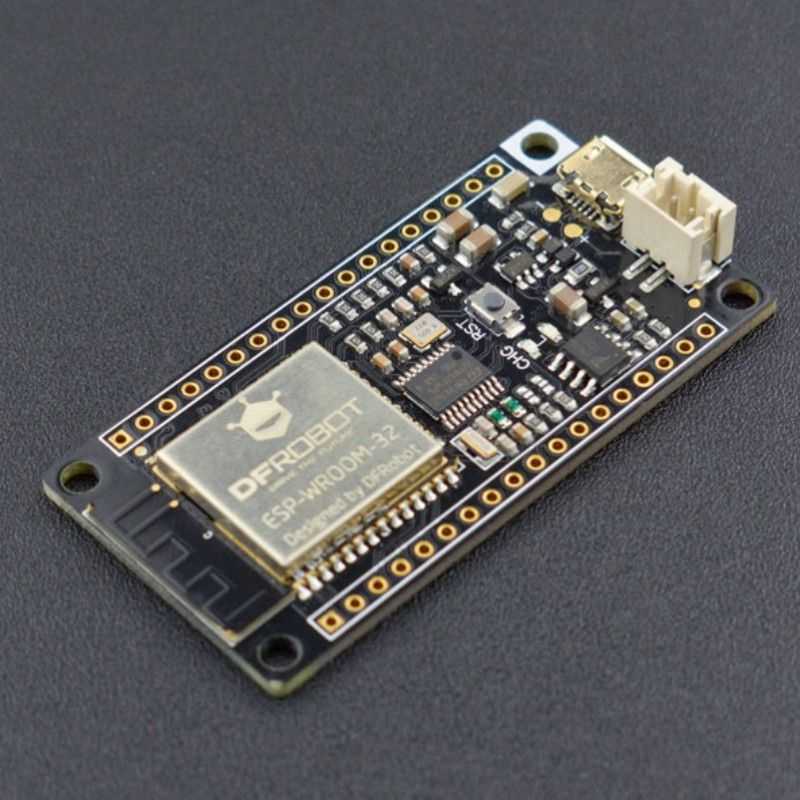
\includegraphics[ width=0.75\linewidth, valign=t]{Bilder/Firebeetle.jpg}
    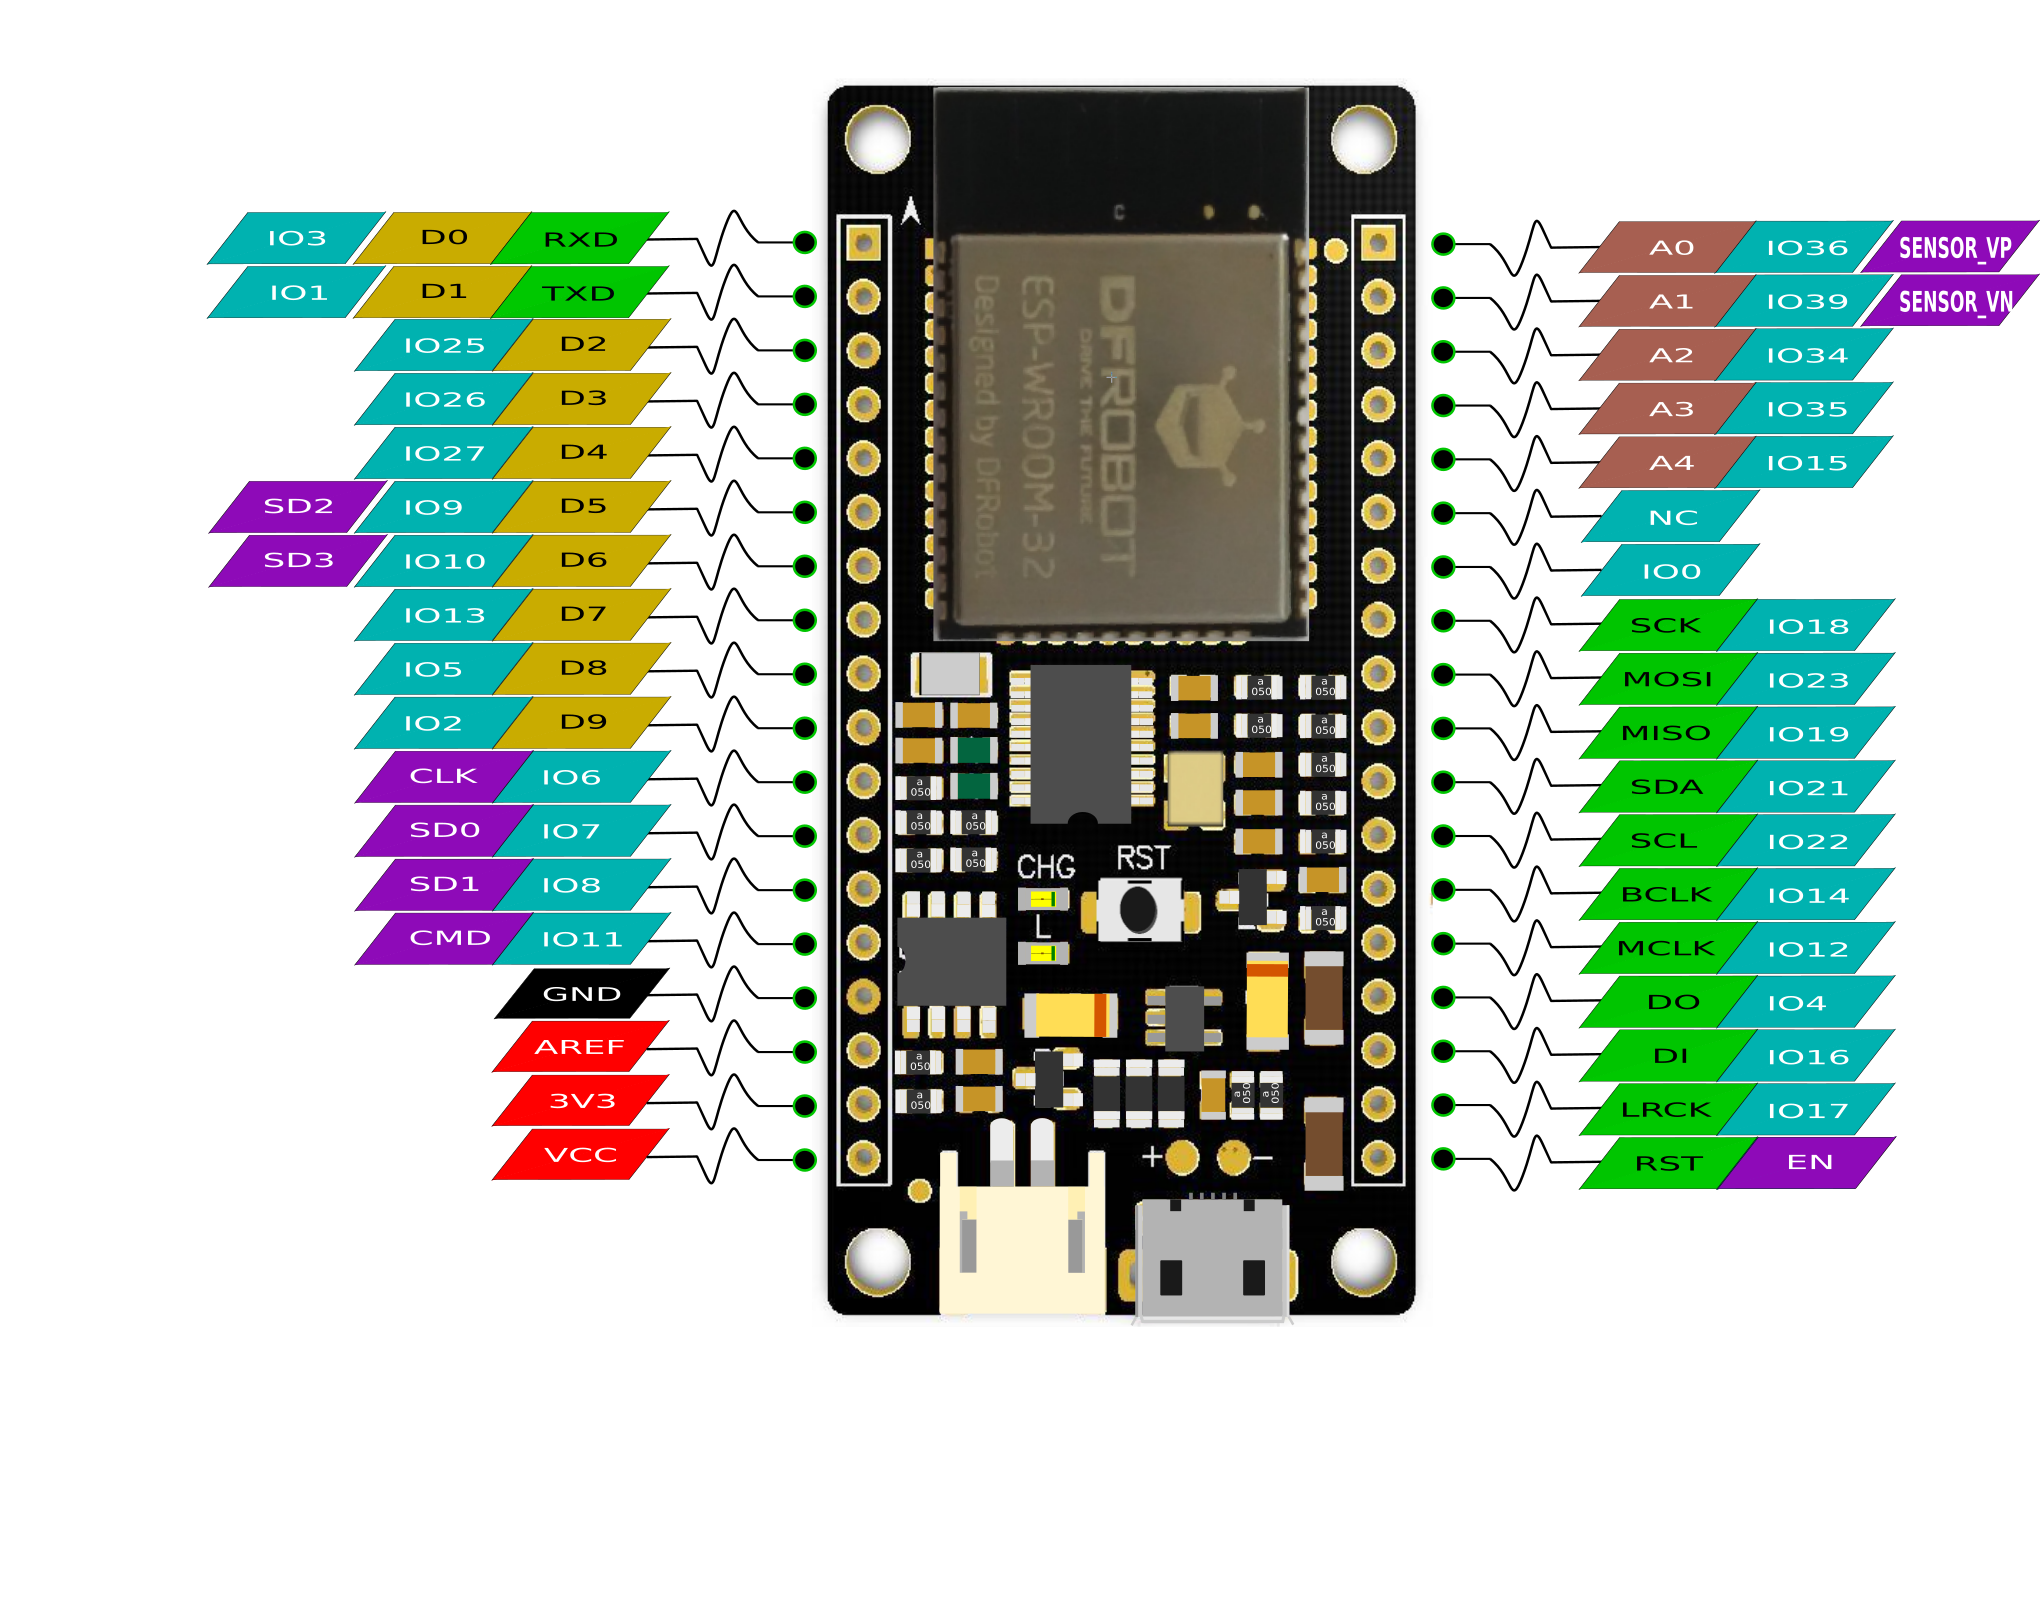
\includegraphics[width=17cm, left]{Bilder/FireBeetleBoard.png}
    \captionsetup{justification=centering}
    \captionof{figure}{Anschlüsse des Firebeetle}
	\end{minipage}%
	\begin{minipage}[t]{0.5\linewidth}
	Als Basis für alle Sensoren ist der Firebeetle\footnotemark \cite{firebeetle} sehr gut geeignet. Leider sind noch nicht alle Bibliotheken, welche für den Vorgänger ESP8266 existieren, für den ESP32 adaptiert worden. Vor einem Projekt sollte man also prüfen ob die benötigten Bibliotheken in der richtigen Version vorhanden sind.
\end{minipage}
\footnotetext{https://www.bastelgarage.ch/firebeetle-esp32-iot-mikrocontroller-mit-wifi}
\section{Arduino}
\begin{minipage}[t]{0.5\linewidth}\label{arduino}
	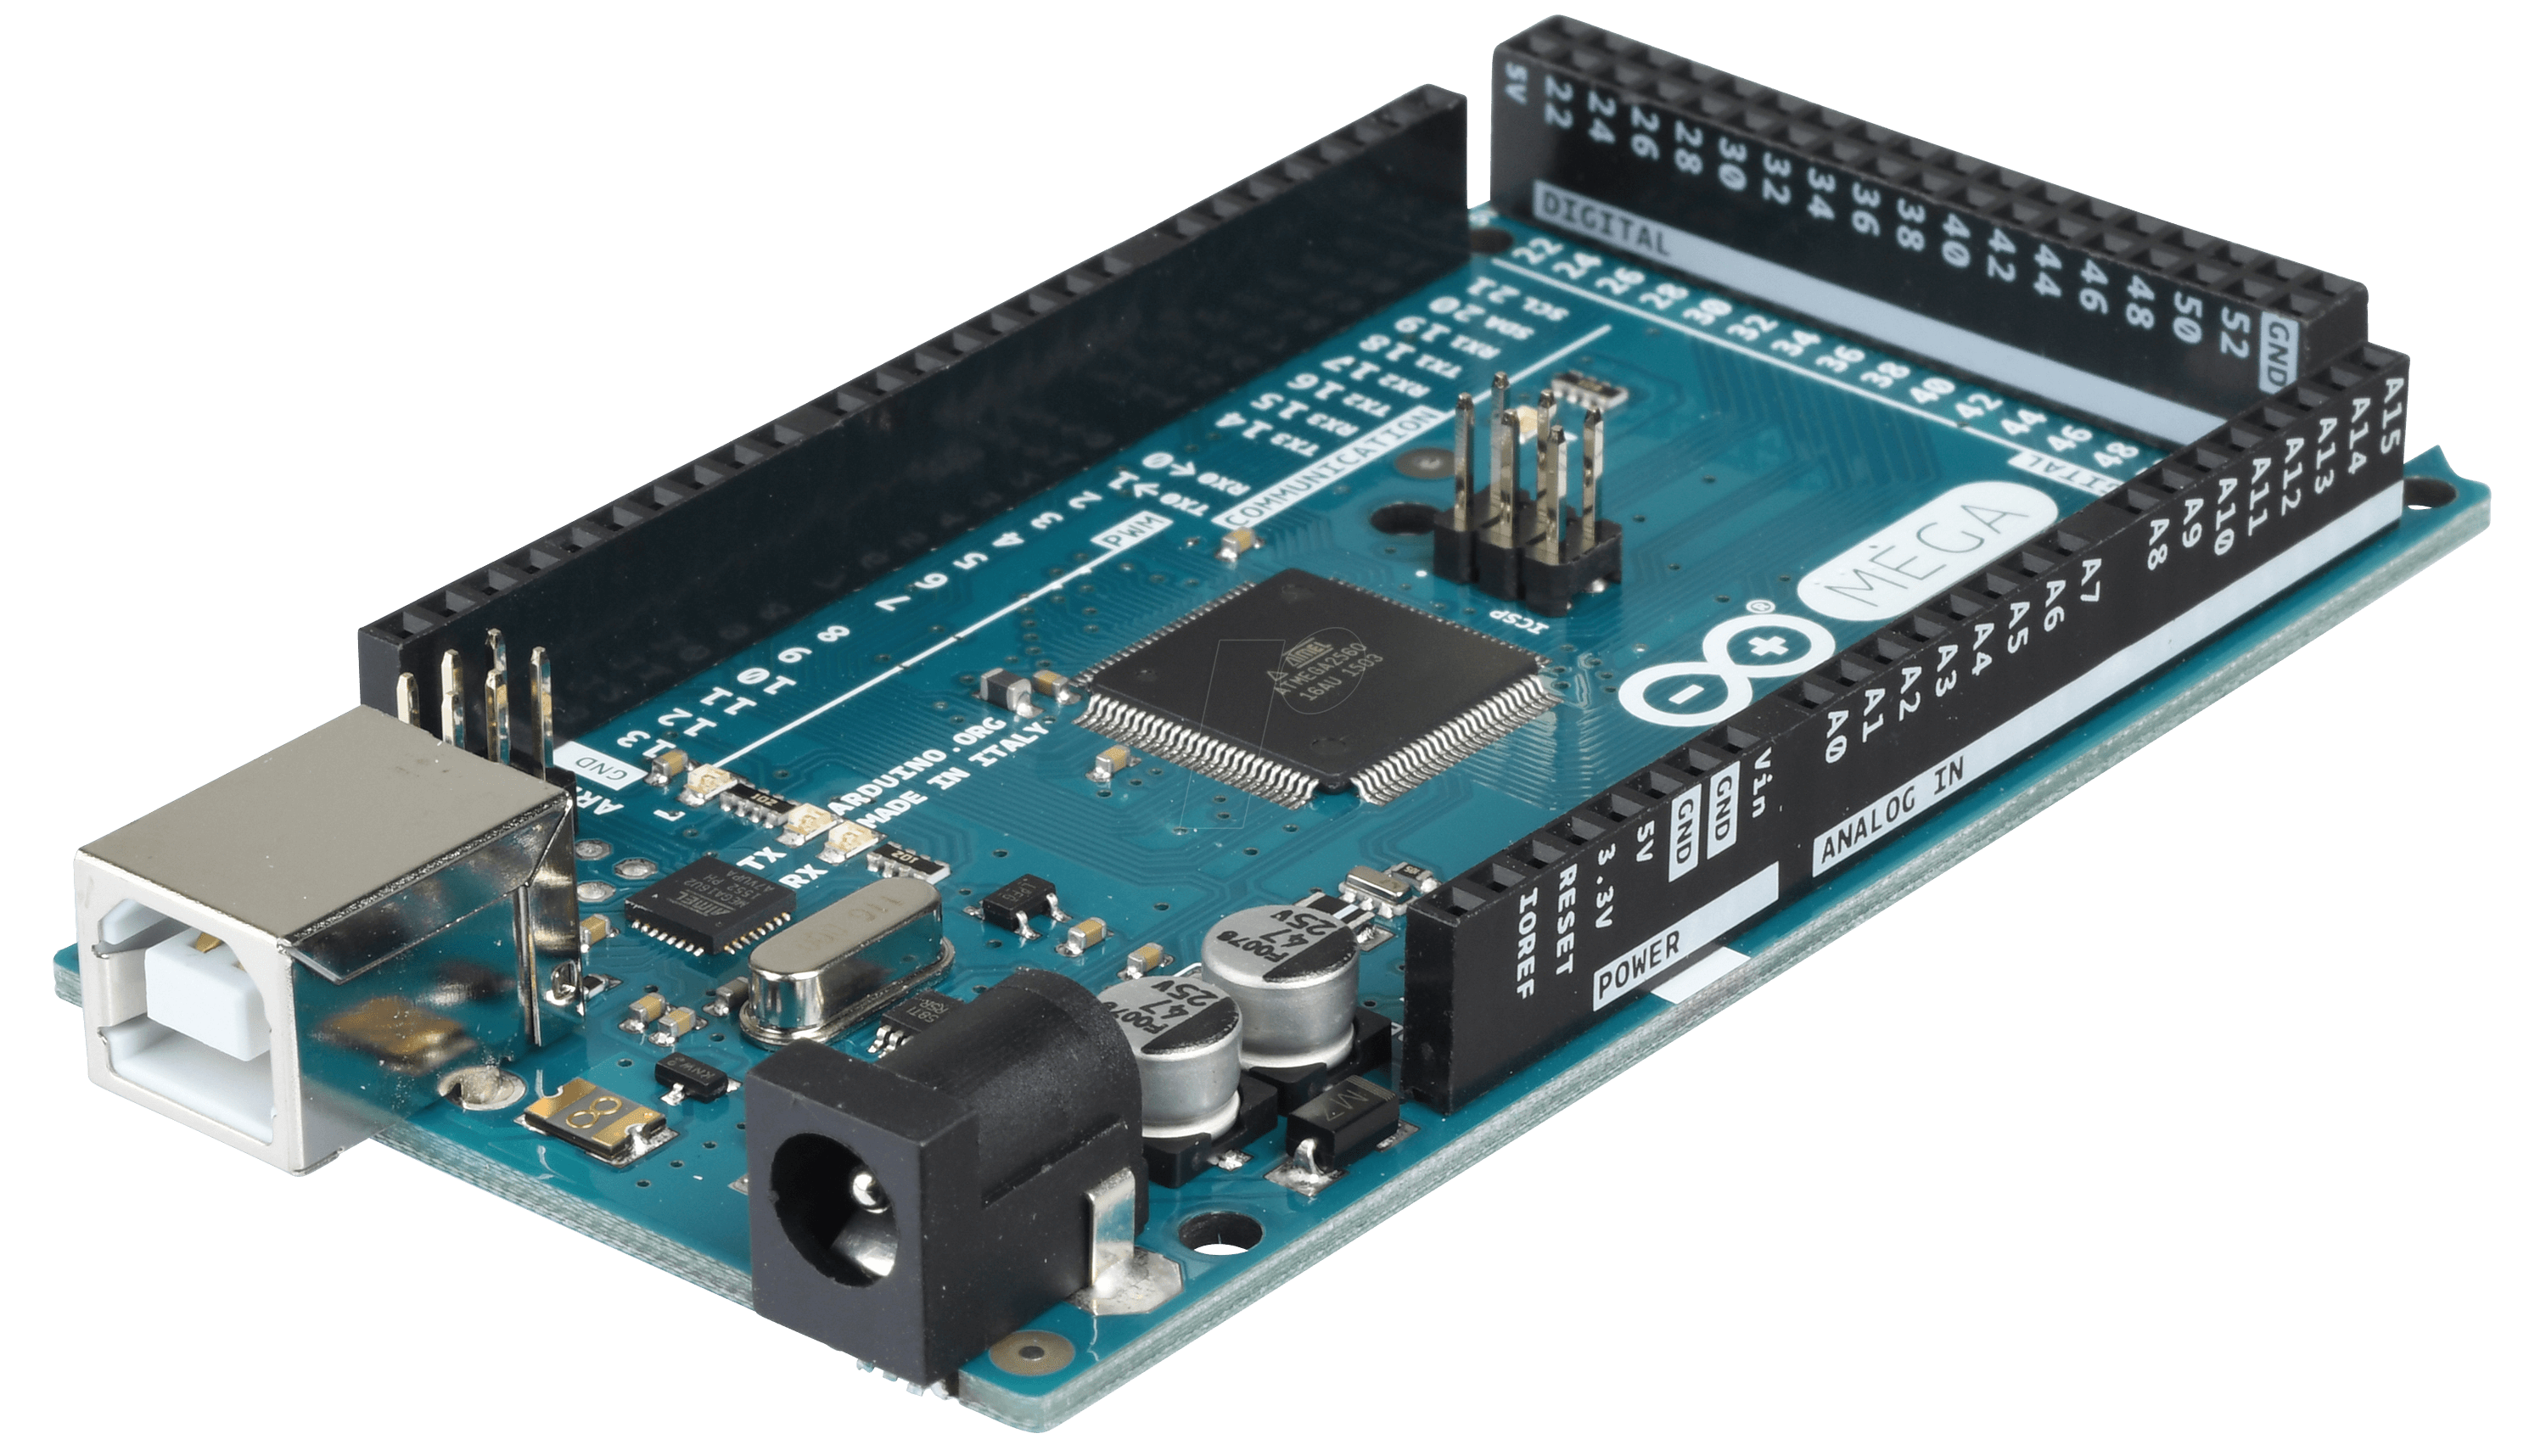
\includegraphics[ width=0.75\linewidth, valign=t]{Bilder/ARDUINO_MEGA_A01.png}
    \captionsetup{justification=raggedright}
    \captionof{figure}{Arduino Mega}
    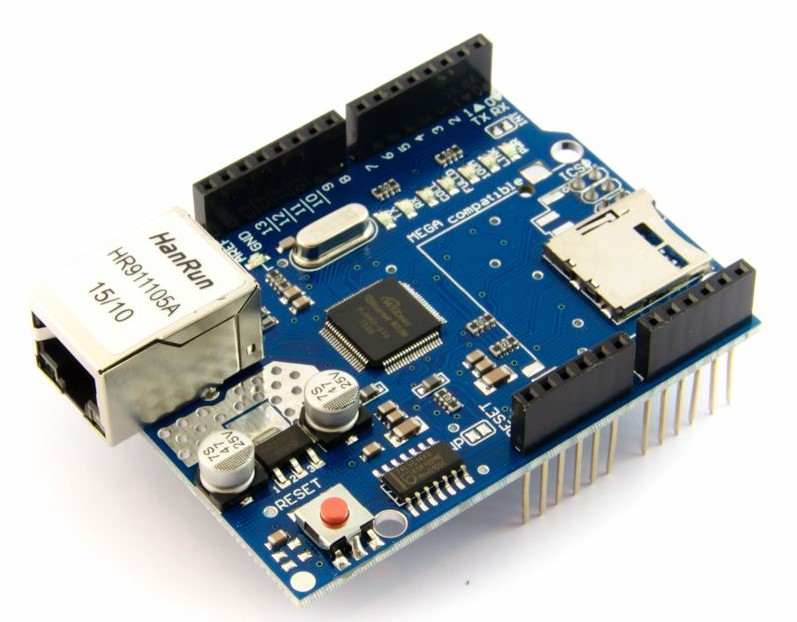
\includegraphics[ width=0.75\linewidth, valign=t]{Bilder/EthernetShield.jpg}
     \captionsetup{justification=raggedright}
    \captionof{figure}{Ethernet Shield für den Arduino}
	\end{minipage}%
	\begin{minipage}[t]{0.5\linewidth}
	Ein Arduino Mega \footnotemark zusammen mit dem Ethernet Shield (Shield = Erweiterung) W5100 \footnotemark bildet das MQTT Gateway. Für die Kommunikation mit den Sensoren ist ein NRF24 Funkmodul zuständig [\ref{nrf24Radio}].
\end{minipage}
\footnotetext{https://store.arduino.cc/arduino-mega-2560-rev3}
 \footnotetext{https://www.bastelgarage.ch/ethernet-shield-spi-w5100-fur-arduino}
\section{Raspberry Pi}
\begin{minipage}[t]{0.5\linewidth}\label{raspberry}
	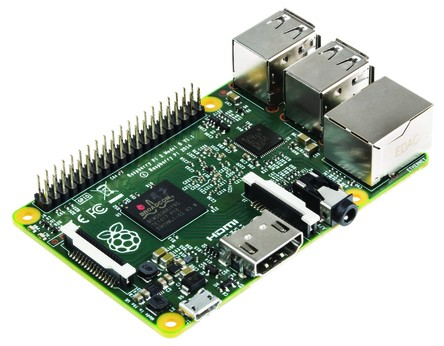
\includegraphics[ width=0.75\linewidth, valign=t]{Bilder/RaspberryPi2.jpg}
    \captionsetup{justification=raggedright}
    \captionof{figure}{Raspberry Pi 2}
	\end{minipage}%
	\begin{minipage}[t]{0.5\linewidth}
	Die Software für die Speicherung der Daten und die Visualisierung wurde auf einem Raspberry Pi 2 installiert \footnotemark. Obwohl dieses Model bereits älter ist und nur 1GB Ram besitzt ist die Leistung für dieses Projekt ausreichend.
\end{minipage}
 \footnotetext{https://www.pi-shop.ch/raspberry-pi-2-model-b-v1-2-1-gb-ram}
 \section{Sensoren}
 \subsection{Temperatur und Luftfeuchtigkeit}
 \subsubsection{DHT22}\label{DHT22}
\begin{minipage}[t]{0.5\linewidth}
		\centering
    		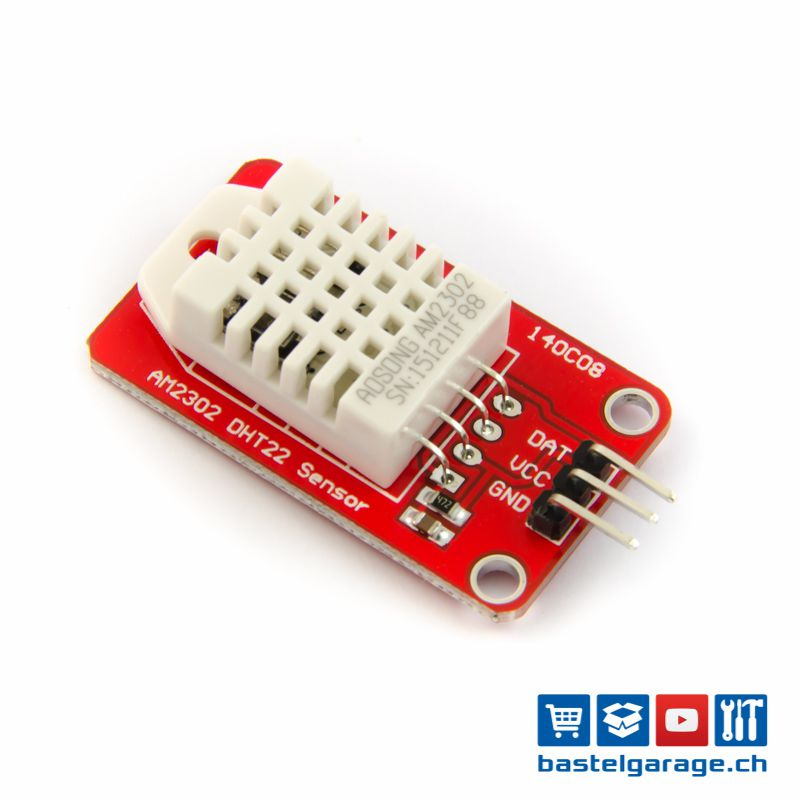
\includegraphics[width=\compImgSize, left, valign=t]{Bilder/DHT22.jpg}
    		 \captionsetup{justification=raggedright}
    		\captionof{figure}{Temperatur und Luftfeuchtigkeitsmesser DHT22}
	\end{minipage}
	\begin{minipage}[t]{0.5\linewidth}
	Der DHT22 \footnotemark ist eine Kombination aus Lufttemperatur und Luftfeuchtigkeitssensor. Gegenüber dem DHT11 ist er präziser, kostet aber auch mehr.
\end{minipage}
\footnotetext{https://www.bastelgarage.ch/dht22-temperatur-und-luftfeuchtigkeitssensor-steckbar}

\subsubsection{DHT11}\label{DHT11}
	\begin{minipage}[t]{0.5\linewidth}
		\centering
		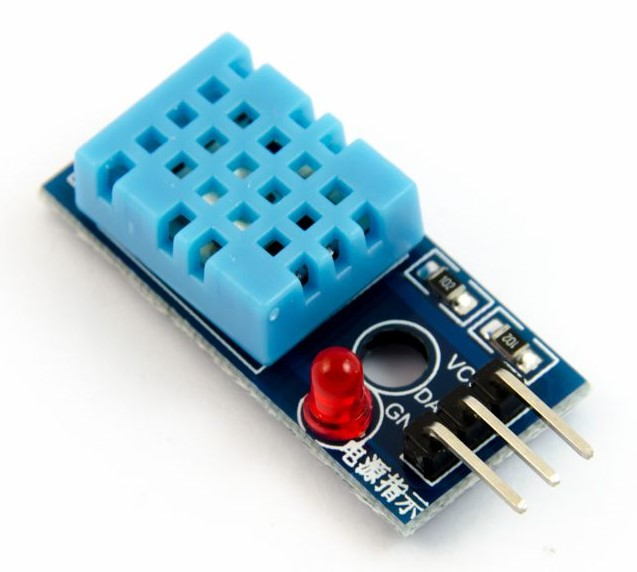
\includegraphics[ width=\compImgSize, left, valign=t]{Bilder/DHT11.jpg} 
		 \captionsetup{justification=raggedright}
		 \captionof{figure}{DHT11 Luft- und Feuchtigkeitssensor}
	\end{minipage}
	\begin{minipage}[t]{0.5\linewidth}
	Als Alternative zu dem oben genannten DHT22 gibt es eine billigere Variante mit dem Namen DHT11 \footnotemark.
	Der DHT11 Sensor hat eine geringere Auflösung als der DHT22, ist ansonsten aber gleich anwendbar.
	\end{minipage}
	 \footnotetext{https://www.bastelgarage.ch/dht11-temperatur-und-luftfeuchtigkeitssensor}

\subsection{Bodenfeuchtigkeit}\label{moistV1.2}
\begin{minipage}[t]{0.5\linewidth}
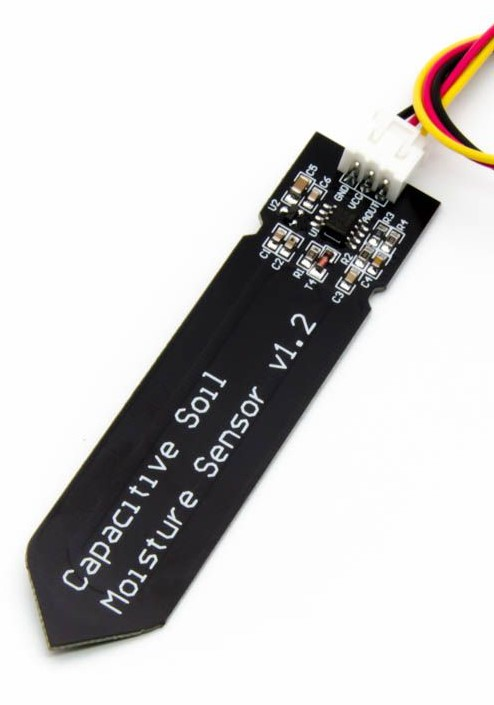
\includegraphics[width=\compImgSize, left, valign=t]{Bilder/Soil-2.jpg}%
\captionof{figure}{Bodenfeuchtesensor V1.2}\label{labelname}
\end{minipage}
\begin{minipage}[t]{0.5\linewidth}
Der Bodenfeuchtesensor V1.2 \footnotemark nimmt die Messung kapazitiv vor, d.h. es werden keine leitenden Kontakte in das Erdreich benötigt. Dadurch ist dieser Sensor keinem Verschleiss unterworfen. Die Messung erfolgt analog und muss danach in die gewünschte Masseinheit umgerechnet werden.
\end{minipage}
 \footnotetext{https://www.bastelgarage.ch/bauteile/sensoren/kapazitiver-bodenfeuchtesensor-v1-2}
 
\subsection{Funk}
\begin{minipage}[t]{0.5\linewidth}\label{nrf24Radio}
        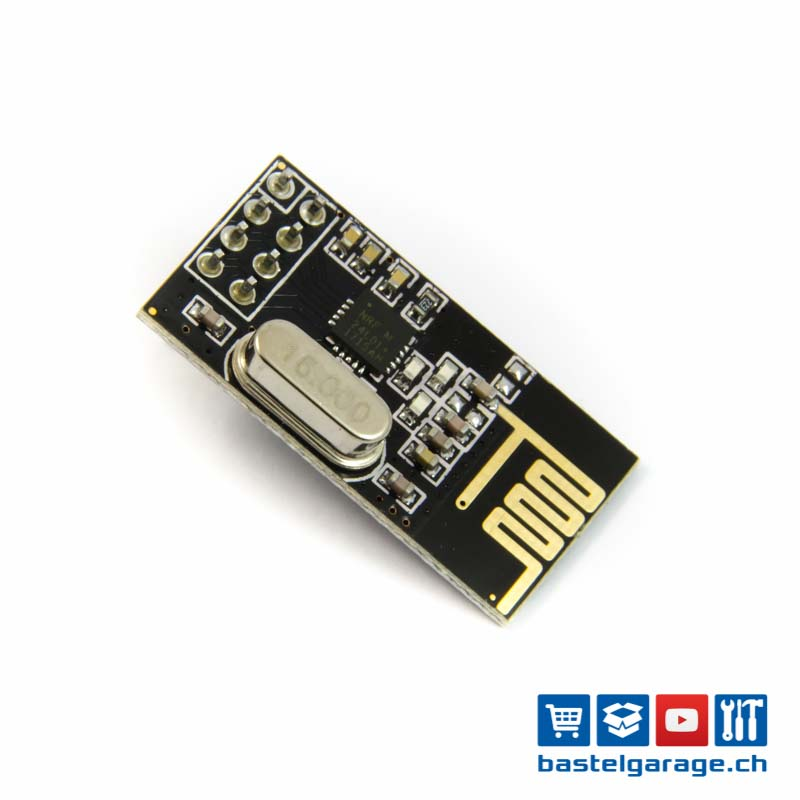
\includegraphics[width=\compImgSize, valign=t]{Bilder/NRF24.jpg} % second figure itself
        \captionsetup{justification=raggedright}
        \captionof{figure}{NRF24L01+ Funkmodul}
\end{minipage}
\begin{minipage}[t]{0.5\linewidth}
Das Funkmodul NRF24L01+ \footnotemark funkt im 2,4GHz Band und benötigt wenig Strom bei einer guten Reichweite. Der Preis ist sehr niedrig für diesen Baustein, allerdings ist die Anwendung aufwendiger als bei anderen Funkprotokollen.
\end{minipage}
\footnotetext{https://www.bastelgarage.ch/bauteile/funk-wireless-lora/nrf24l01-wireless-funk-modul-2-4ghz}

% List of Figures
\listoffigures
% List of Tables
\begingroup
\let\clearpage\relax
\listoftables
% Glossary
\printglossary
% Bibliography

\renewcommand\bibname{Linkverzeichnis}
\begin{thebibliography}{99}\label{links}
   \bibitem{whyHmac}What is HMAC Authentication and why is it useful?\break \url{https://www.wolfe.id.au/2012/10/20/what-is-hmac-authentication-and-why-is-it-useful/}
    \bibitem{esp32-hmac}ESP32 Arduino: Applying the HMAC SHA-256 mechanism\break \url{https://techtutorialsx.com/2018/01/25/esp32-arduino-applying-the-hmac-sha-256-mechanism/}
    \bibitem{mbedTLS} mbed TLS, Library für den ESP32 welche viele Kryptografische Funktionen implementiert\break \url{https://tls.mbed.org/}
    \bibitem{spi} Standard Bibliothek sowohl für den Arduino wie auch den ESP32 welche die Kommunikation mit anderen Komponenten, in diesem Fall die einzelnen Sensor Module, übernimmt\break \url{https://www.arduino.cc/en/Reference/SPI}
    \bibitem{rfh24} Bibliothek für den nRF24L01 Baustein welche sowohl auf dem Arduino als auch dem ESP32 verwendbar ist \break \url{https://github.com/nRF24/RF24}
    \bibitem{hmacOnline}Online HMAC Code Generator\break \url{https://www.freeformatter.com/hmac-generator.html#ad-output}
    \bibitem{nrf24}NRF24L01+ Funkmodul Treiber für Arduino und ESP32\break \url{http://tmrh20.github.io/RF24/index.html}
    \bibitem{dht} Bibliothek für die beiden Sensoren DHT11 und DHT22 sowohl für Arduino als auch den ESP32 \break \url{https://github.com/adafruit/DHT-sensor-library}
    \bibitem{espressif}Herstellerseite Espressif für den ESP32\break \url{https://www.espressif.com/en/products/hardware/esp32/overview}
    \bibitem{arduino}Arduino Herstellerseite mit der gleichnamigen IDE und vielen Bibliotheken und Tutorials\break \url{https://www.arduino.cc/}
    \bibitem{firebeetle}Herstellerseite des Firebeetle Mikrokontrollers\break \url{https://www.dfrobot.com/product-1590.html}
    \bibitem{uploader}Erweiterung für die Arduino IDE um Dateien in den Flash Speicher des ESP32 zu laden \break \url{https://github.com/me-no-dev/arduino-esp32fs-plugin}
    \bibitem{pubsubclient}Arduino Client for MQTT \break \url{https://github.com/knolleary/pubsubclient}
    \bibitem{ethernet}Arduino Ethernet library\break \url{https://www.arduino.cc/en/Reference/Ethernet}
    \bibitem{nrf24Arduino}Arduino driver for nRF24L01 2.4GHz Wireless Transceiver \break \url{https://github.com/maniacbug/RF24}
    \bibitem{cryptosuite}SHA1 / SHA256 and HMAC-SHA1 / HMAC-SHA256 Hash library\break \url{http://spaniakos.github.io/Cryptosuite/}
    \bibitem{mosquitto}Open Source MQTT Broker Mosquitto\break \url{https://mosquitto.org/}
    \bibitem{telegraf} Server Agent welcher Daten aus verschiedenen Quellen sammelt und weiterleitet \break \url{https://www.influxdata.com/time-series-platform/telegraf/}
    \bibitem{telegrafmqtt}MQTT Plugin für Telegraf\break \url{https://github.com/influxdata/telegraf/tree/master/plugins/inputs/mqtt_consumer}
    \bibitem{influx} InfluxDB, Open Source Zeitreihendatenbank \break \url{https://www.influxdata.com/products/influxdb-overview/}
    \bibitem{influxAuth}Authentication and authorization in InfluxDB\break \url{https://docs.influxdata.com/influxdb/v1.7/administration/authentication_and_authorization/}
    \bibitem{grafana} Datenvisualierungs-Software Grafana\break \url{https://grafana.com/}
    \bibitem{grafanaDashboard}Grafana Graph Panel \break \url{https://grafana.com/docs/features/panels/graph/}
    \bibitem{radioPower}Design of Wireless Sensors for IoT with Energy Storage and Communication Channel Heterogeneity\break \url{https://www.mdpi.com/1424-8220/19/15/3364/pdf}
    \bibitem{connect}Kafka Connect MQTT Connector \break  \url{https://docs.confluent.io/current/connect/kafka-connect-mqtt/}
    \bibitem{espssl}ESP32 MQTT Library \break \url{https://github.com/espressif/esp-mqtt}
    \bibitem{mosquittoSSL}Mosquitto SSL Configuration -MQTT TLS Security\break \url{http://www.steves-internet-guide.com/mosquitto-tls/}
  \end{thebibliography}
%Index
\addcontentsline{toc}{chapter}{Index}
%\printindex
% Appendices
\endgroup
\end{document}
